%# -*- coding: utf-8 -*-
% !TeX encoding = UTF-8 Unicode
% !TeX spellcheck = en_US
% !TeX TS-program = xelatex
%~ \XeTeXinputencoding "UTF-8"
% vim:ts=4:sw=4
%
% 以上设定默认使用 XeLaTex 编译,并指定 Unicode 编码,供 TeXShop 自动识别

%\documentclass[a4paper,10pt,twocolumn]{article}
\documentclass[letter,11pt,onecolumn]{book}
%\documentclass[letter,11pt,onecolumn,adobefonts]{ctexbook}

\newcommand{\doctitle}{mrnative -- run native software in an Hadoop/HPC environment}
\newcommand{\docauthor}{傅允辉}
\newcommand{\dockeywords}{Linux, mrnative, Hadoop}
\newcommand{\docsubject}{}

\newcommand{\usedefaultTWO}[2]{
\if\relax\detokenize{#2}\relax
  #1
\else
  #2
\fi
}

\newcommand{\usedefaultTHREE}[3]{
\if\relax\detokenize{#3}\relax
  \usedefaultTWO{#1}{#2}
\else
  #3
\fi
}

% 用于接受从 xelatex/pdflatex 通过参数 -jobname 传入的参数来判定编译何种语言的版本。
% \cnt 的三个参数分别为 en/zh/tw 的内容
\newcommand{\cnt}[3]{{#1}{#2}{#3}}
%\newcommand{\cnt}[3]{#1} % default en
\usepackage{ifthen}
\ifthenelse{\equal{\detokenize{lang-zh}}{\jobname}}{
  \renewcommand{\cnt}[3]{\usedefaultTWO{#1}{#2}}
}{
  \ifthenelse{\equal{\detokenize{lang-tw}}{\jobname}}{
    \renewcommand{\cnt}[3]{\usedefaultTHREE{#1}{#2}{#3}}
  }{
    % default en
    \renewcommand{\cnt}[3]{#1}
    %\renewcommand{\cnt}[3]{#2}
  }
}

\newcommand{\cnts}[3]{{#1} {#2}}

% 根据配置来设置中文环境
\newcommand\usefontspeczh[1]{#1} % use fontspec for zh_CN
\newcommand\charsetzhcn[1]{#1} % the charset encoding for zh_CN
\newcommand\formatzhcn[1]{#1} % the page format for zh_CN
\cnt{
\renewcommand\usefontspeczh[1]{}
\renewcommand\charsetzhcn[1]{}
\renewcommand\formatzhcn[1]{}
}{
%\renewcommand\usefontspeczh[1]{}
%\renewcommand\charsetzhcn[1]{}
%\renewcommand\formatzhcn[1]{}
}{
%\renewcommand\usefontspeczh[1]{}
%\renewcommand\charsetzhcn[1]{}
%\renewcommand\formatzhcn[1]{}
}
%# -*- coding: utf-8 -*-
% !TeX encoding = UTF-8 Unicode
% !TeX spellcheck = en_US
% !TeX TS-program = xelatex
%~ \XeTeXinputencoding "UTF-8"
% vim:ts=4:sw=4
%
% 以上设定默认使用 XeLaTex 编译,并指定 Unicode 编码,供 TeXShop 自动识别

% 使用 LaTex 写中文的配置模板
%\documentclass[12pt]{article}

%\newcommand{\doctitle}{Peer-to-Peer Communication Across Network Address Translators}
%\newcommand{\doctitle}{穿越NAT的点对点通信}
%\newcommand{\docauthor}{Bryan Ford \& Pyda Srisuresh \& Dan Kegel}
%\newcommand{\dockeywords}{NAT穿越, 点对点, NAT Traversal, Peer-to-Peer}
%\newcommand{\docsubject}{NAT穿越}
%\newcommand\usefontspeczh[1]{#1} % use fontspec for zh_CN
%\newcommand\charsetzhcn[1]{#1} % the charset encoding for zh_CN
%\newcommand\formatzhcn[1]{#1} % the page format for zh_CN

\newcommand\mymainfont{DejaVu Serif}%{Times New Roman} %{DejaVu Serif}
\newcommand\mymonofont{DejaVu Sans Mono}%{FreeMono} %{WenQuanYi Micro Hei Mono} %{Monaco}
\newcommand\myboldfont{WenQuanYi Micro Hei Mono}%{AR PL UKai CN}%{YaHei Consolas Hybrid}%{黑体}%{標楷體}
\newcommand\mysansfont{DejaVu Sans}%{FreeSans}
\newcommand\myitalicfont{DejaVu Serif}%{Times New Roman} %{Garamond}

\newcommand\mycjkboldfont{WenQuanYi Micro Hei Mono}%{Adobe Heiti Std}%{AR PL UKai CN}%{YaHei Consolas Hybrid}%{黑体}%{標楷體}
\newcommand\mycjkitalicfont{全字庫正楷體} %{Adobe Kaiti Std}
\newcommand\mycjkmainfont{AR PL UMing CN}%{Adobe Song Std}%{仿宋}%{宋体}%{新宋体}%{文鼎PL新宋}%
\newcommand\mycjksansfont{Adobe Ming Std}
\newcommand\mycjkmonofont{WenQuanYi Micro Hei Mono}%{AR PL UMing CN}%{WenQuanYi Micro Hei Mono}

\usepackage{ifthen}
\usepackage{ifpdf}
\usepackage{ifxetex}
\usepackage{ifluatex}

\usepackage{color}
\usepackage[rgb,x11names]{xcolor} %must before tikz, x11names defines RoyalBlue3


\usefontspeczh{

\usepackage[cm-default]{fontspec} % XeLaTex 配合 fontspec

\charsetzhcn{
  %\renewcommand\mycjkmainfont{AR PL UMing CN}%{仿宋}%{宋體}%{新宋體}%{文鼎PL新宋}%

  \ifxetex    % xelatex

    %\usepackage[cm-default]{fontspec} % XeLaTex 配合 fontspec 可以非常方便地设置字体。[cm-default]选项主要用来解决使用数学环境时数学符号不能正常显示的问题
    %\usepackage{xltxtra,xunicode} %这行和上行 \usepackage[cm-default]{fontspec} 解决公式不正常的问题.但是打开后有些如 itemize 的点不能显示。

    \usepackage[
        BoldFont, % 允許粗體
        SlantFont,        % 允許斜體
        %CJKsetspaces,
        CJKchecksingle
        ]{xeCJK}
    \defaultfontfeatures{Mapping=tex-text} %如果沒有它,會有一些 tex 特殊字符無法正常使用,比如連字符。

    \XeTeXlinebreaklocale "zh"                      % 重要,使得中文可以正確斷行!
    \XeTeXlinebreakskip = 0pt plus 1pt minus 0.1pt  %

    \setCJKmainfont[BoldFont=\mycjkboldfont, ItalicFont=\mycjkitalicfont]{\mycjkmainfont}
    \setCJKsansfont{\mycjksansfont}%{Adobe Ming Std} %{AR PL UMing CN} %{Microsoft YaHei}
    \setCJKmonofont{\mycjkmonofont}

  \fi


\formatzhcn{
    %\newfontfamily{\j}{Osaka}       % 设置特殊字符,这里是为日文准备的特殊字体。没有该字体,所以关闭。

    \setlength{\parindent}{2.04em}  %设置首行缩进。只有中文才打开。
    \linespread{1.3}                % 设置行距

    %\definecolor{bisque}{rgb}{.996,.891,.755}
    %\pagecolor{bisque} % 设置背景颜色

    % 设置原文照排环境的字体
    \makeatletter
    \def\verbatim@font{\sffamily\small}
    \makeatother

    % 将默认的英文重定义为中文
    \renewcommand{\contentsname}{\cnt{Content}{目录}{目錄}}
    \renewcommand{\listfigurename}{\cnt{List of Figures}{插图目录}{插圖目錄}}
    \renewcommand{\listtablename}{\cnt{List of Tables}{表格目录}{表格目錄}}
    \renewcommand{\indexname}{\cnt{Index}{索引}{索引}}
    \renewcommand{\tablename}{\cnt{Table}{表}{表}}
    \renewcommand{\figurename}{\cnt{Figure}{图}{圖}}
    \renewcommand{\appendixname}{\cnt{Chapter}{附录}{附錄}}

    % article
    %\renewcommand{\refname}{\cnt{Bibliography}{参考文献}{參考文獻}}
    %\renewcommand{\abstractname}{\cnt{Abstract}{摘要}{摘要}}

    % book
    %\renewcommand{\chaptername}{\cnt{Chapter}{章节}{章節}}
    %\renewcommand{\bibname}{\cnt{Bibliography}{参考}{參考}}

    %\renewcommand{\IEEEkeywordsname}{\cnt{Keywords}{关键词}{關鍵詞}}


    % 设置页眉页脚
    \usepackage[pagestyles,compact]{titlesec} % 定制页眉页脚
    \newpagestyle{main}{%
        \sethead[$\cdot$~\thepage~$\cdot$][][\thesection\quad%
        \sectiontitle]{\thesection\quad\sectiontitle}{}{%
            $\cdot$~\thepage~$\cdot$}
        \setfoot{}{}{}\headrule}
        \pagestyle{main}
        \renewpagestyle{plain}{\sethead{}{}{}\setfoot{}{}{}}
    \pagestyle{plain}

    %% 设置chapter, section与subsection的格式
    \titleformat{\chapter}{\centering\huge}{\textbf{第\thechapter{}章}}{1em}{\textbf}
    \titleformat{\section}{\centering\LARGE}{\textbf{\thesection}}{1em}{\textbf}
    \titleformat{\subsection}{\Large}{\textbf{\thesubsection}}{1em}{\textbf}

    %% For LaN
    \newcommand{\LaN}{L{\scriptsize\hspace{-0.47em}\raisebox{0.23em}{A}}\hspace{-0.1em}N}

    %% 去掉表头中的冒号
    \makeatletter
        \long\def\@makecaption#1#2{%
            \vskip\abovecaptionskip
            \sbox\@tempboxa{#1~~#2}%
            \ifdim \wd\@tempboxa >\hsize
                #1~~#2\par
            \else
                \global \@minipagefalse
                \hb@xt@\hsize{\hfil\box\@tempboxa\hfil}%
            \fi
            \vskip\belowcaptionskip}
    \makeatother
} % formatzhcn

} % \charsetzhcn

\setmonofont[Scale=0.8]{\mymonofont} % 英文等宽字体
\setsansfont{\mysansfont}       % 英文无衬线字体
%\setmainfont{\mymainfont}        % 英文衬线字体, setmainfont=setromanfont
\setromanfont[Mapping=tex-text,  % 沿用 LaTex 的一些习惯的标点转换,例如 en-dash 以两个减号表示
    Ligatures={Required,Common}, % 如果此字体内置 Ligatures 定义则启用
    ItalicFont={\myitalicfont},  % 斜体用 Times Italic,严格来说只有拉丁子母有斜体。
    BoldFont={\myboldfont}]      % 粗体用字体
    {\mymainfont}                % 内文使用字体, Linux 下用 "fc-list :lang=zh-cn" 列出支持的中文字体
} % \usefontspeczh

% 设置中文状态下, 恢复 lstlisting 的 mono 字体
\usepackage[T1]{fontenc}
\DeclareTextCommandDefault{\nobreakspace}{\leavevmode\nobreak\ } % EU1 encoding setup has changed \nobreakspace from being an encoding-independent command to an encoding-dependent command, but without setting up a default definition so it works in all encodings.

\usepackage{dtklogos} % \LaTeXe 等
% XeTeX logo
%\def\XeTeX{\leavevmode
%    \setbox0=\hbox{X\lower.5ex\hbox{\kern-.15em\reflectbox{E}}\kern-.1667em \TeX}%
%    \dp0=0pt\ht0=0pt\box0}

% the algorithm2e package
\makeatletter
\newif\if@restonecol
\makeatother
\let\algorithm\relax
\let\endalgorithm\relax
\usepackage[ruled,vlined]{algorithm2e} %\usepackage[figure,ruled,vlined]{algorithm2e}

\usepackage{url}
\usepackage{array}

\usepackage{courier}
\usepackage{listings} % list the source code
\definecolor{ForestGreen}{rgb}{0.13,0.55,0.13}

\lstset{
    language=C,
    captionpos=b, %t,
    tabsize=3,
    basicstyle=\footnotesize\ttfamily, %basicstyle=\ttfamily\normalsize, %basicstyle=\small\ttfamily, %\normalfont\ttfamily, % \large\ttfamily, % \small\ttfamily, % \footnotesize\ttfamily, % \scriptsize\ttfamily, % Standardschrift,
    numbers=left,               %左侧显示行号 往左靠,还可以为right,或none,即不加行号
    stepnumber=1,               %若设置为2,则显示行号为1,3,5,即stepnumber为公差,默认stepnumber=1
    %numberstyle=\tiny,         %行号字体用小号
    numberstyle={\color[RGB]{0,192,192}\tiny} ,%设置行号的大小,大小有tiny,scriptsize,footnotesize,small,normalsize,large等
    numbersep=8pt,              %设置行号与代码的距离,默认是5pt
    breaklines=true,            %对过长的代码自动换行
    showstringspaces=false,     %不显示代码字符串中间的空格标记
    frame=shadowbox, %=lines,                    %把代码用带有阴影的框圈起来
    stringstyle=\ttfamily,      % 代码字符串的特殊格式
    commentstyle=\color{ForestGreen}, %\color{red!50!green!50!blue!50}, %浅灰色的注释
    rulesepcolor=\color{red!20!green!20!blue!20}, %代码块边框为淡青色
    keywordstyle=\color{blue!90}\bfseries,        %代码关键字的颜色为蓝色,粗体
    backgroundcolor=\color[rgb]{1,1,1},%\color[RGB]{245,245,244},   %代码背景色 \color[rgb]{0.91,0.91,0.91}
    framextopmargin=2pt,framexbottommargin=2pt,abovecaptionskip=-3pt,belowcaptionskip=3pt,
%    xleftmargin=4em,xrightmargin=4em, % 设定listing左右的空白
%    %language={[ISO]C++},       %language为,还有{[Visual]C++}
%    alsolanguage=Java,
%    %alsolanguage=[ANSI]C,      %可以添加很多个alsolanguage,如alsolanguage=matlab,alsolanguage=VHDL等
%    %alsolanguage= tcl,
%    alsolanguage= XML,
%    keepspaces=true,            %
%    breakindent=22pt,           %
%    breakindent=4em,            %
%    showspaces=false,           %
%    flexiblecolumns=true,       %
%    breakautoindent=true,       %
%    aboveskip=1em,              %代码块边框
%    %% added by http://bbs.ctex.org/viewthread.php?tid=53451
%    fontadjust,
%    texcl=true,
%    escapeinside=``,            %在``里显示中文
%    %escapebegin=\begin{CJK*}{GBK}{hei},escapeend=\end{CJK*},
%    % 设定中文冲突,断行,列模式,数学环境输入,listing数字的样式
%    extendedchars=false,columns=flexible,
%    mathescape=false,
%    % numbersep=-1em,
    emph={label}
}

\renewcommand{\ttdefault}{pcr}

\definecolor{darkgreen}{cmyk}{0.7, 0, 1, 0.5}
\definecolor{darkblue}{rgb}{0.1, 0.1, 0.5}
\lstdefinelanguage{diff}
{
    keywords={+, -, \ , @@, diff, index, new},
    sensitive=false,
    morecomment=[l][""]{\ },
    morecomment=[l][\color{darkgreen}]{+},
    morecomment=[l][\color{red}]{-},
    morecomment=[l][\color{darkblue}]{@@},
    morecomment=[l][\color{darkblue}]{diff},
    morecomment=[l][\color{darkblue}]{index},
    morecomment=[l][\color{darkblue}]{new},
    morecomment=[l][\color{darkblue}]{similarity},
    morecomment=[l][\color{darkblue}]{rename},
}

\lstdefinelanguage{JavaScript}{
  keywords={typeof, new, true, false, catch, function, return, null, catch, switch, var, if, in, while, do, else, case, break},
  keywordstyle=\color{blue}\bfseries,
  ndkeywords={class, export, boolean, throw, implements, import, this},
  ndkeywordstyle=\color{darkgray}\bfseries,
  identifierstyle=\color{black},
  sensitive=false,
  comment=[l]{//},
  morecomment=[s]{/*}{*/},
  %commentstyle=\color{purple}\ttfamily,
  commentstyle=\color{green}\ttfamily,
  stringstyle=\color{red}\ttfamily,
  morestring=[b]',
  morestring=[b]"
}

\usepackage{tabularx} % long table
\usepackage{booktabs,longtable} % table in seperate pages.


\ifxetex % xelatex
\else
    %The cmap package is intended to make the PDF files generated by pdflatex "searchable and copyable" in acrobat reader and other compliant PDF viewers.
    \usepackage{cmap}%
\fi
% ============================================
% Check for PDFLaTeX/LaTeX
% ============================================
\newcommand{\outengine}{xetex}
\newif\ifpdf
\ifx\pdfoutput\undefined
  \pdffalse % we are not running PDFLaTeX
  \ifxetex
    \renewcommand{\outengine}{xetex}
  \else
    \renewcommand{\outengine}{dvipdfmx}
  \fi
\else
  \pdfoutput=1 % we are running PDFLaTeX
  \pdftrue
  \usepackage{thumbpdf}
  \renewcommand{\outengine}{pdftex}
  \pdfcompresslevel=9
\fi
\usepackage[\outengine,
    bookmarksnumbered, %dvipdfmx
    %% unicode, %% 不能有unicode选项,否则bookmark会是乱码
    colorlinks=true,
    citecolor=red,
    urlcolor=blue,        % \href{...}{...} external (URL)
    filecolor=red,      % \href{...} local file
    linkcolor=black, % \ref{...} and \pageref{...}
    breaklinks,
    pdftitle={\doctitle},
    pdfauthor={\docauthor},
    pdfsubject={\docsubject},
    pdfkeywords={\dockeywords},
    pdfproducer={Latex with hyperref},
    pdfcreator={pdflatex},
    %%pdfadjustspacing=1,
    pdfborder=1,
    pdfpagemode=UseNone,
    pagebackref,
    bookmarksopen=true]{hyperref}

% --------------------------------------------
% Load graphicx package with pdf if needed 
% --------------------------------------------
\ifxetex    % xelatex
    \usepackage{graphicx}
\else
    \ifpdf
        \usepackage[pdftex]{graphicx}
        \pdfcompresslevel=9
    \else
        \usepackage{graphicx} % \usepackage[dvipdfm]{graphicx}
    \fi
\fi

%% \DeclareGraphicsRule{.jpg}{eps}{.bb}{}
%% \DeclareGraphicsRule{.png}{eps}{.bb}{}
\graphicspath{{./} {figures/}}
\usepackage{flafter} % 防止图形在文字前

%%%% 字体:
%Adobe Heiti Std 和 Adobe Song Std是砖头公司出的两款超pp的字体,有人把它们用在latex排版中,效果超级好。
%windows版在 Program Files/Adobe/Acrobat 8.0/Resource/CIDFont 下。

%sudo mkdir /usr/share/fonts/adobe
%sudo cp DIR2adobefonts/*.otf /usr/share/fonts/adobe
%sudo chmod 644 /usr/share/fonts/adobe/*.otf # 当前用户读写,当前组用户读写,其他用户只读

%cd /usr/share/fonts/adobe/
%sudo mkfontscale #(创建fonts.scale文件,控制字体旋转缩放)
%sudo mkfontdir #(创建fonts.dir文件,控制字体粗斜体产生)
%sudo fc-cache -fv # (建立字体缓存信息,也就是让系统认识认识)
%fc-list :lang=zh-cn # 看看装上没


%安装 LaTeX+XeTeX环境的过程, 你也使用Emacs来编辑TeX文件的话, 那么一定要安上AUCTeX这个扩展
%sudo apt-get install texlive texlive-latex-extra texlive-xetex lmodern # 首先是LaTeX与XeTeX的安装

%sudo apt-get install auctex

%安装好以后, 重点是配置.emacs文件, 因为AUCTeX本身是不支持通过xelatex编译的.
%;; AUCTeX
%(defun auctex ()
  %(add-to-list 'TeX-command-list '("XeLaTeX" "%`xelatex%(mode)%' %t; %`xelatex%(mode)%' %t" TeX-run-TeX nil t)) ;; 这里我编译了两次
    %(setq TeX-command-default "XeLaTeX") ;; 设定默认编译命令为XeLaTeX
    %(setq TeX-save-query nil)            ;; 保存之前不询问
    %(setq TeX-show-compilation t))       ;; 在新窗口显示编译过程
%(add-hook 'LaTeX-mode-hook 'auctex)

%(custom-set-variables
 %'(TeX-output-view-style (quote (("^dvi$nnnnnnn" ("^landscape$" "^pstricks$\\|^pst-\\|^psfrag$") "%(o?)dvips -t landscape %d -o && gv %f") ("^dvi$" "^pstricks$\\|^pst-\\|^psfrag$" "%(o?)dvips %d -o && gv %f") ("^dvi$" ("^a4\\(?:dutch\\|paper\\|wide\\)\\|sem-a4$" "^landscape$") "%(o?)xdvi %dS -paper a4r -s 0 %d") ("^dvi$" "^a4\\(?:dutch\\|paper\\|wide\\)\\|sem-a4$" "%(o?)xdvi %dS -paper a4 %d") ("^dvi$" ("^a5\\(?:comb\\|paper\\)$" "^landscape$") "%(o?)xdvi %dS -paper a5r -s 0 %d") ("^dvi$" "^a5\\(?:comb\\|paper\\)$" "%(o?)xdvi %dS -paper a5 %d") ("^dvi$" "^b5paper$" "%(o?)xdvi %dS -paper b5 %d") ("^dvi$" "^letterpaper$" "%(o?)xdvi %dS -paper us %d") ("^dvi$" "^legalpaper$" "%(o?)xdvi %dS -paper legal %d") ("^dvi$" "^executivepaper$" "%(o?)xdvi %dS -paper 7.25x10.5in %d") ("^dvi$" "." "%(o?)xdvi %dS %d") ("^pdf$" "." "acroread %o %(outpage)") ("^html?$" "." "netscape %o")))))

%最后那个有点长, 主要是没有找到合适的方法像添加XeLaTeX一样只需要写新增的条目, 所以这里就把原有的和修改以后的都写了出来. 其实只改了一个地方, 已经用蓝色标注出来了, 就是在使用C-c C-v预览PDF文件的时候使用什么软件来打开. 我这里就是acroread, 你用的其它的话, 可以相应修改.
%这样修改好以后, 以后就可以直接使用C-c C-c编译, C-c C-v预览, C-c `在错误间跳转了.

%但是TeX Live中的install-info文件会导致源安装AUCTeX的时候失败, 所以如果是先安装的TeX Live, 再安装AUCTeX, 就需要先把TeX Live的install-info"消灭"掉: 
%sudo mv /usr/local/bin/install-info /usr/local/bin/install-info.bak

%-------------------------------------------------------------------
%终于搞定在emacs+auctex中设置xelatex为默认编译命令!

%只要在在~/.emacs中加上

%(add-hook 'LaTeX-mode-hook (lambda()
    %(add-to-list 'TeX-command-list '("XeLaTeX" "%`xelatex%(mode)%' %t" TeX-run-TeX nil t))
    %(setq TeX-command-default "XeLaTeX")
    %(setq TeX-save-query  nil )
    %(setq TeX-show-compilation t)
    %))

%第一行参考auctex的手册auctex.pdf,版本是11.84 ;
%(add-to-list 'TeX-command-list '("XeLaTeX" "%`xelatex%(mode)%' %t" TeX-run-TeX nil t)) 会在Command 这一栏中增加了XeLaTeX这一项命令;
%(setq TeX-command-default "XeLaTeX")  则使得以后用C-c C-c就是默认用xelatex 命令编译tex文档;
%(setq TeX-save-query  nil ) 这一行不用确认保存就开始执行编译;
%(setq TeX-show-compilation t)  这一行是看到编译的滚动信息。
%现在还是在latex-mode下配置,下一步看能否在pdflatex-mode 下配置。


%(add-to-list 'TeX-command-list '("XeLaTeX" "%`xelatex%(mode)%' %t" TeX-run-TeX nil t)) 这一行中的"%`xelatex%(mode)%' %t"
%写成"xelatex  %t" 已经可以了。



\newcommand\comments[1]{#1}
\renewcommand\comments[1]{}

\usepackage{xcolor}

\usepackage{amssymb}
%\usepackage{amsmath,amsfonts,amsthm}

\usepackage{array}
% table's multirow and multicolumn
\usepackage{multirow}

\usepackage{chapterbib}
\usepackage[sectionbib,super,square,sort&compress]{natbib}

%\usepackage[margin=1.8cm,nohead]{geometry}
\usepackage[margin=0.8in,nohead]{geometry}
%\usepackage[top=1in,bottom=1in,left=1.25in,right=1.25in]{geometry} % 设置页边距
%\setlength{\belowcaptionskip}{1em} % 设置caption之后的距离

%opening
\title{\doctitle}
\author{\docauthor}
%\date{2014-03}

\begin{document}

\maketitle
\tableofcontents


%# -*- coding: utf-8 -*-
% !TeX encoding = UTF-8 Unicode
% !TeX spellcheck = en_US
% !TeX TS-program = xelatex
%~ \XeTeXinputencoding "UTF-8"
% vim:ts=4:sw=4
%
% 以上设定默认使用 XeLaTex 编译,并指定 Unicode 编码,供 TeXShop 自动识别

\chapter{Introduction}

There're three types of environment be supported by the software,
which are single host bash, hadoop, and myhadoop.

In hadoop environment, the system will need HDFS to store both the data and executable for all of nodes involved.
\begin{itemize}
  \item executable: such as ns2 C++ binary and its support files
  \item data: config files and TCL scripts for the specific simulation
\end{itemize}
Once a node start to run the simulation, the map-reduce script should load the binary files from HDFS to local host first,
then read a global config file for environment settings,
and read a config file for that simulation to continue simulation.

While in myhadoop case, the data and executable are not necessary to be stored in HDFS since there's share file system for the HPC.
But the user should also be warned because some type of network file system (NFS) will downgrade the simulation speed if the simulator write the data to the NFS directly.
One of the trade-off is to copy the config files from the NFS to a directory of local disks and run the simulator on that directory and copy the data back to the NFS after finishing the simulation.

To overcome all of these challenges mentioned above,
we integrate the following functions in the software:
\begin{itemize}
  \item An abstract interface for the file system: it supports copy files, move files, print files on the standard output, find files etc. So that the software can support local files and HDFS files in a restricted computing environment (we're not system administrator and can't install various file system driver by ourselves.).
  \item use local disks to store data temporally: to speed up the simulation.
\end{itemize}

\begin{figure}\centering
  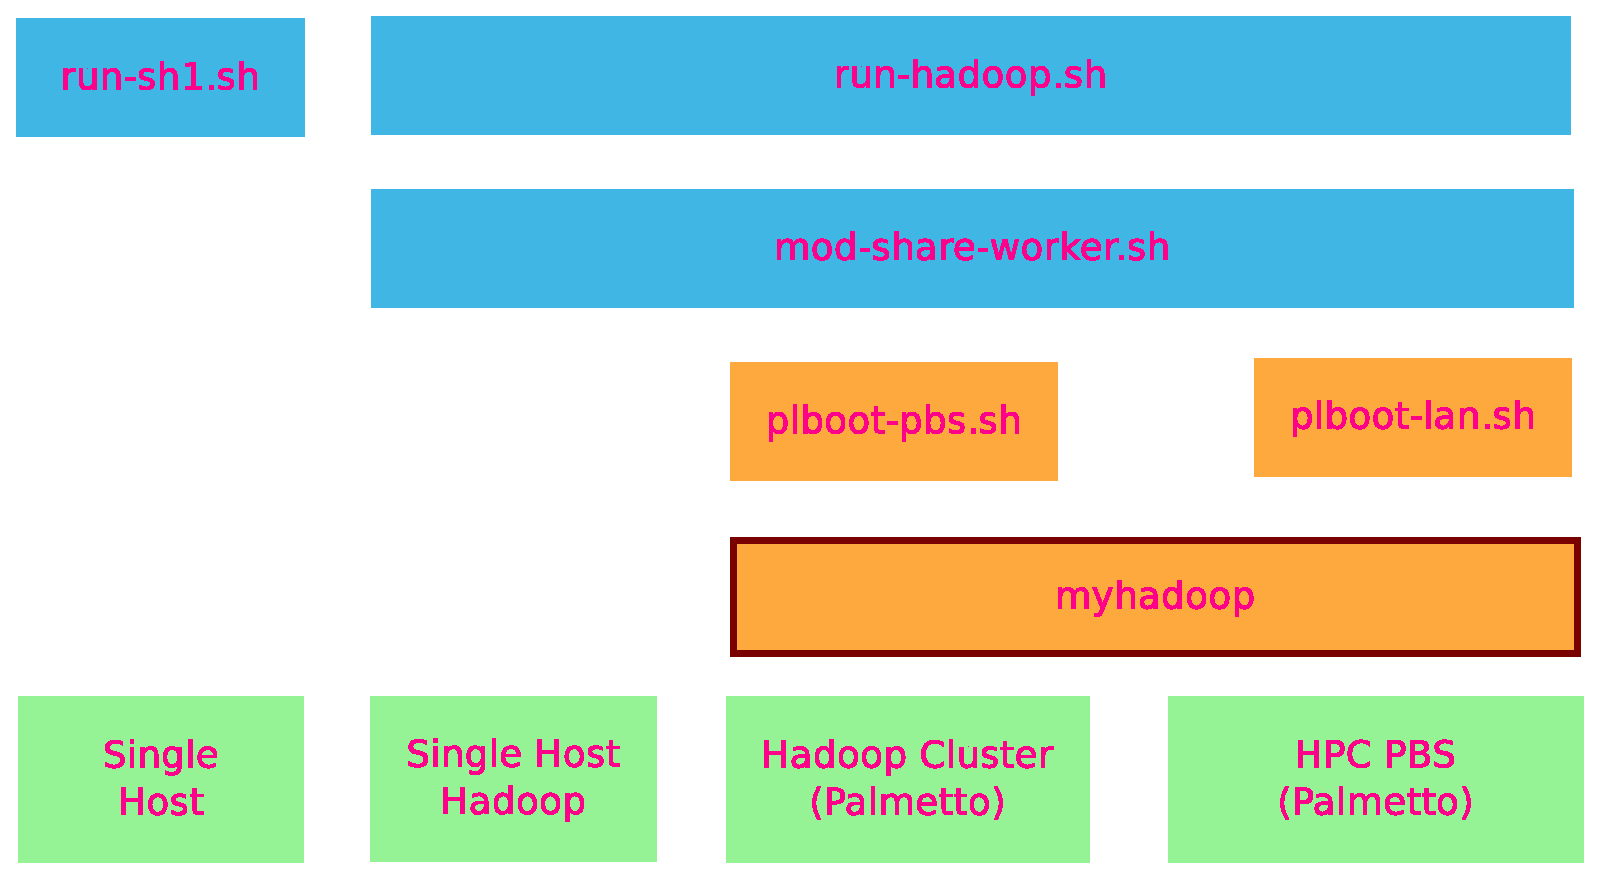
\includegraphics[width=0.9\textwidth]{mrnative-stack}
  \caption{The stack of the mrnative}\label{fig:mrnativestack}
\end{figure}


%# -*- coding: utf-8 -*-
% !TeX encoding = UTF-8 Unicode
% !TeX spellcheck = en_US
% !TeX TS-program = xelatex
%~ \XeTeXinputencoding "UTF-8"
% vim:ts=4:sw=4
%
% 以上设定默认使用 XeLaTex 编译,并指定 Unicode 编码,供 TeXShop 自动识别

\chapter{app-conv2dash}


\section{High Level Design}



\begin{enumerate}
  \item 使用 flowchart 将处理流程初步理清
  \item 使用 \href{http://www.cascading.org/}{Cascading}/MapReduce 实现系统
  \item 测试
\end{enumerate}


\subsection{介绍}

use hadoop to process multimedia contents and simulation

The main tasks we need to contruct the system are:

\begin{enumerate}
  \item transcode task:
  transcode the original media files (*.png, *.flac) to various resolution of the video files,
  generate the .mpd file for DASH

  \item emulation/simulation:
  how to select the parameters for a DASH adaptive algorithm

  \item result process:
  draw the figures?

\end{enumerate}


\subsection{整体结构}
图 \ref{fig:system} 是整个系统的运行框架。
首先,在模块 ``Media Transcode'' 中,用户需要对原始视频源处理,
输出若干解析度和比特率的视频。
这些处理过的视频资源作为输入数据,在 ``Simulation'' 中模拟DASH系统。
在模拟过程所收集到的数据被分析后,重新调整参数,做下次测试。
多轮循环后,输出结果。

\begin{figure}\centering
  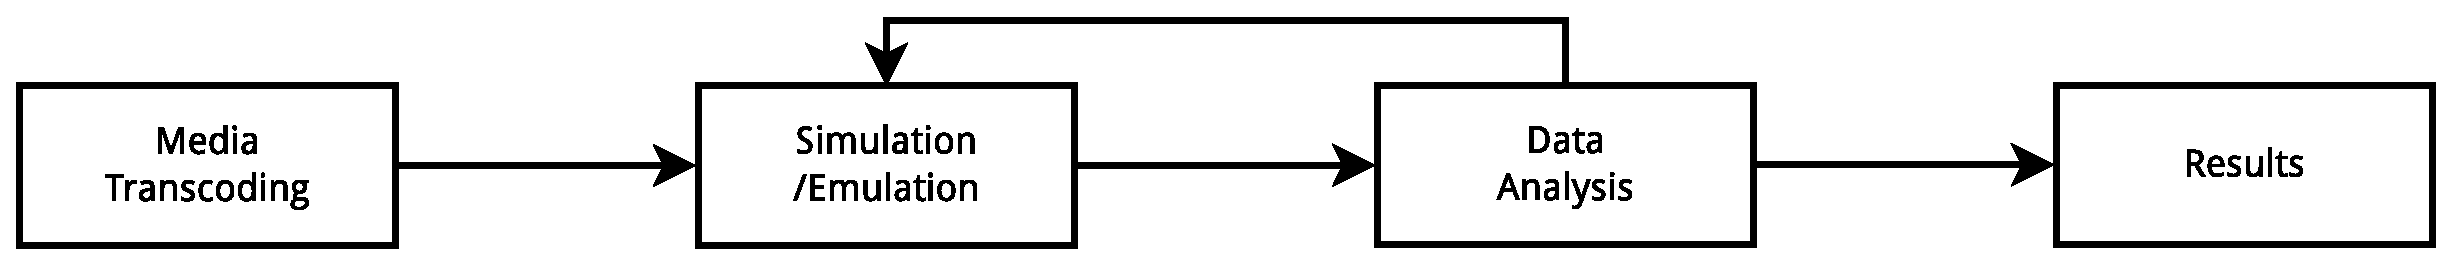
\includegraphics[width=0.9\textwidth]{figures-appconv2dash/flowchart-0-system.eps}
  \caption{The system.}\label{fig:system}
\end{figure}



\subsubsection{模拟参数}

\begin{figure}\centering
  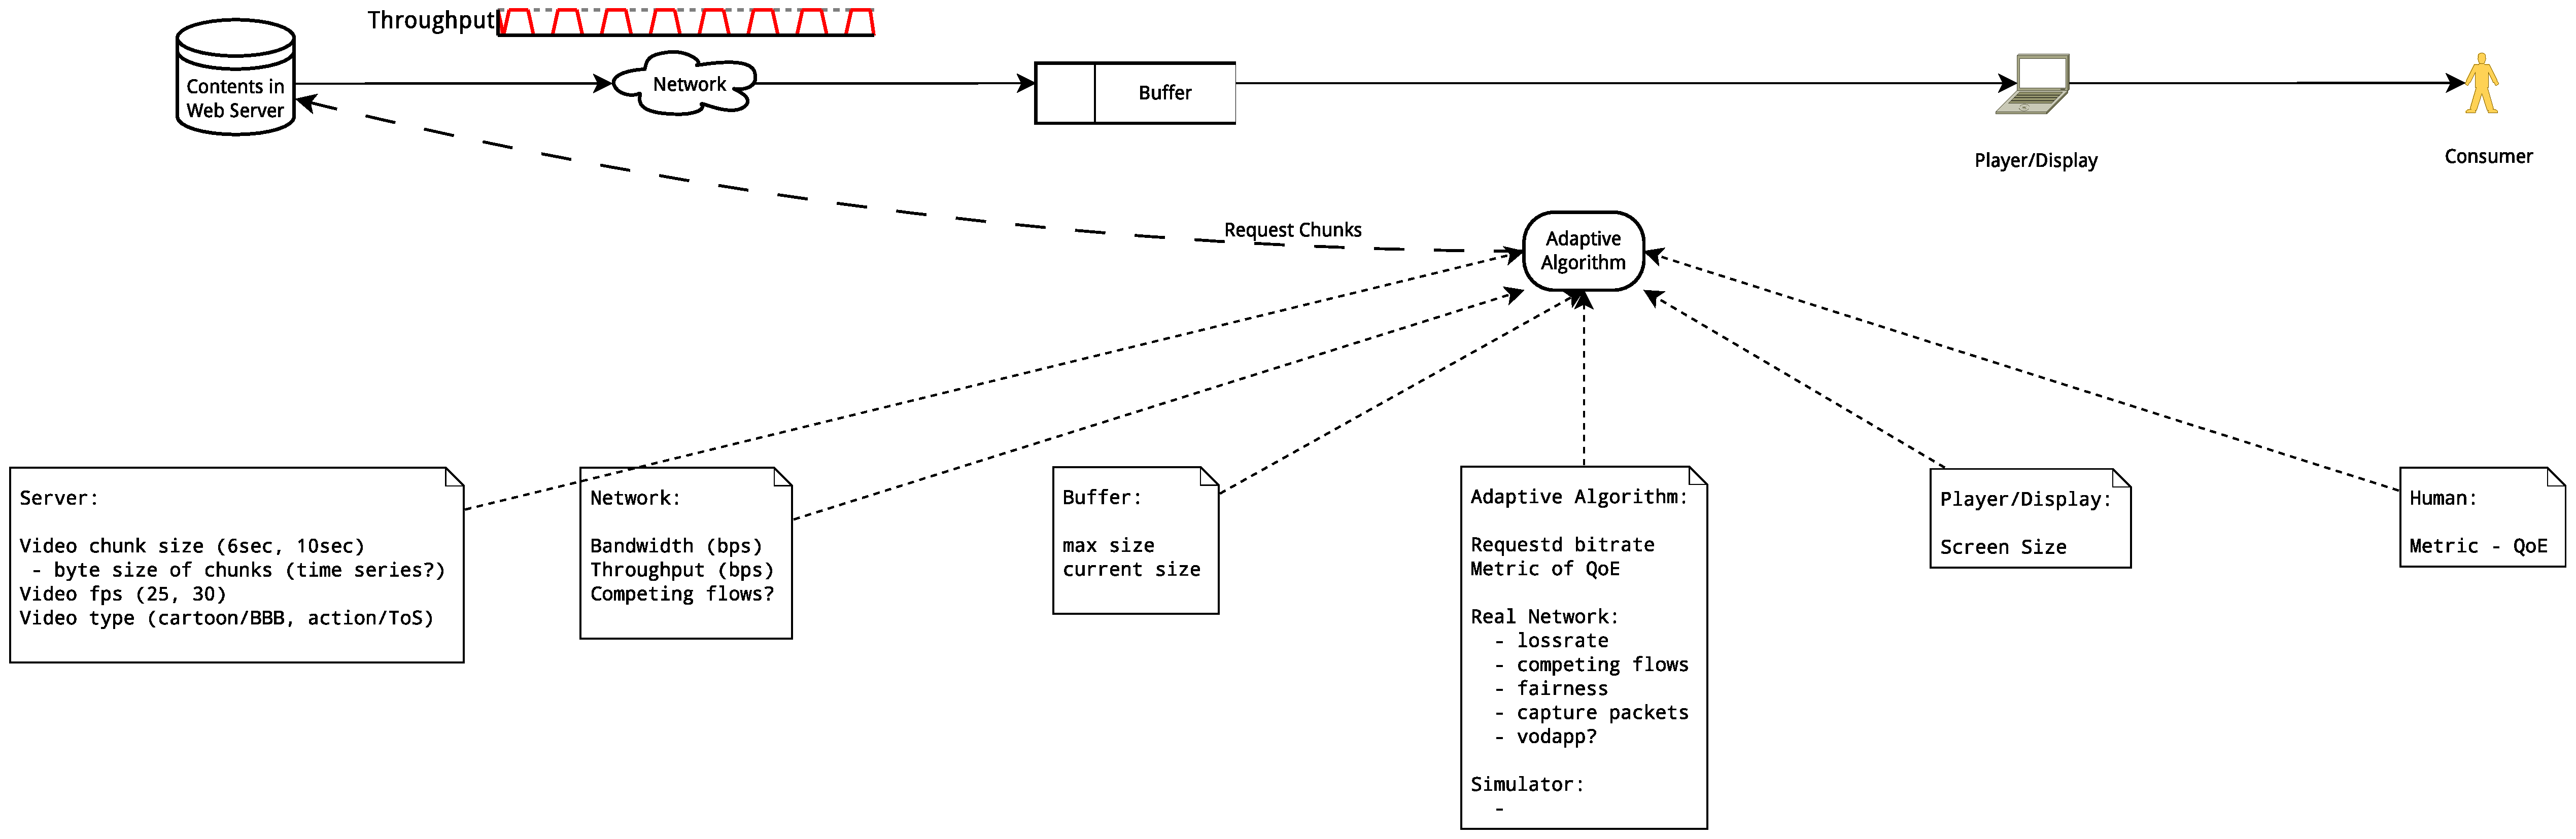
\includegraphics[width=1.1\textwidth]{figures-appconv2dash/dash-parameters.eps}
  \caption{\cnt{The metrics/parameters of the system}{系统参数/测量值}{}.}\label{fig:dashalgoparam}
\end{figure}



\begin{enumerate}
  \item How to evaluate the performance of one video streaming adaptive algorithm? (user metrics, network usages, fairness)
  \item What's the expected results?
  \item training the ML decision algorithm, by metrics(output), parameters(input);
  pre-select parameters for encoder (is it make sense for adaptive algorithm?)
\end{enumerate}




\subsection{用户接口}

用户一般有各种不同内容的视频文件,
需要将其转码到固定几种格式的输出。

基于用户使用习惯,可以将数据接口分为以下几类:

\begin{enumerate}
  \item 输入文件:作为Hadoop 应用程序输入参数的传递;文件的每一行是一个输入视频音频及其相关参数,用于生成一套各种码率的视频;可以在该输入文件中指定若干个视频音频源,输出是多个视频源的结果。
  \item 输出配置:输出是固定格式,包括压缩编码方式、解析度、比的率等;需要在 etc/transcode.conf 中配置
\end{enumerate}




\subsection{视频编码}

图 \ref{fig:vidtranscode} 是一个视频转换编码的流程图。
音频相对占用资源比较小,所以没有并行化。



%\textcolor[HTML]{0000FF}{This text will appear green-colored}

%\textcolor[HTML]{D7FE39}{This text will appear green-colored}


\definecolor{vidtransoriginfile}{HTML}{D7FE39}
\definecolor{vidtranstmpfile}{HTML}{EDE80F}
\definecolor{vidtransfinalfile}{HTML}{FFE985}
\definecolor{vidtransprocess}{HTML}{FEA93E}
\definecolor{vidtransfuncio}{HTML}{DADAFF}
\begin{figure}\centering
  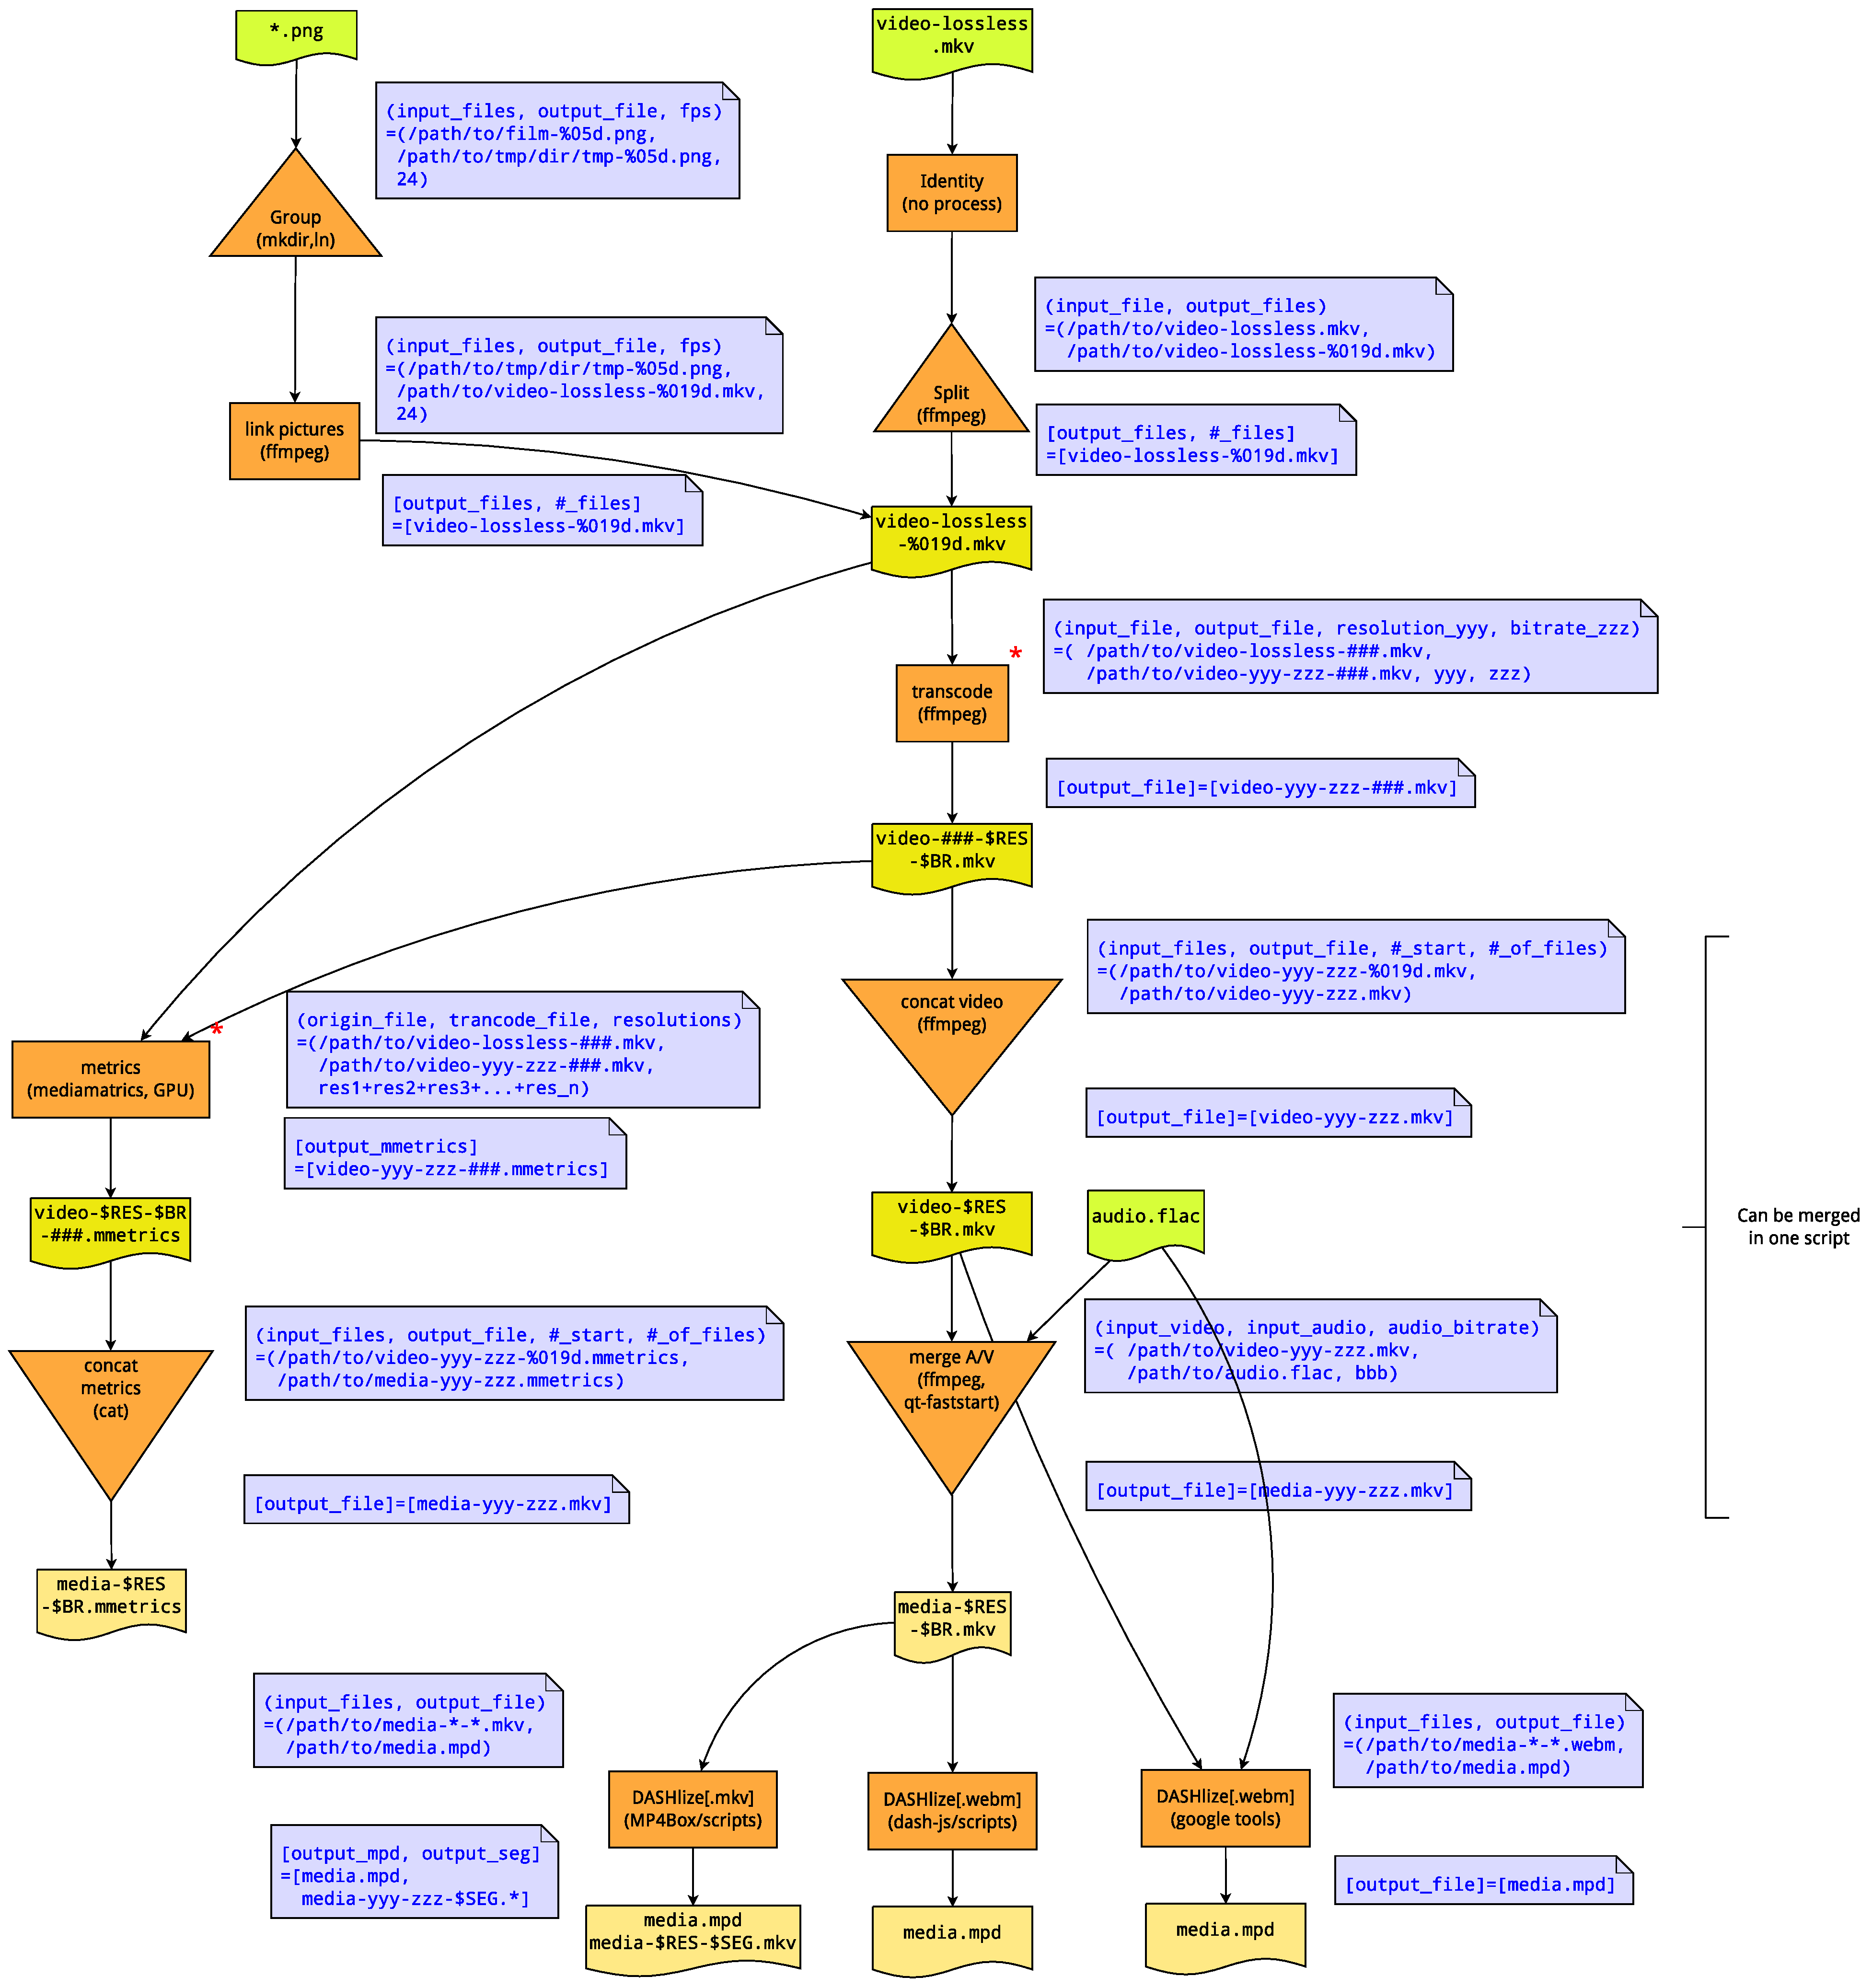
\includegraphics[width=1.1\textwidth]{figures-appconv2dash/flowchart-1-transcode.eps}
  \caption{Data flow for video transcoding.
    The text in \fcolorbox{black}{vidtransoriginfile}{this color} is the original input file.
    The text in \fcolorbox{black}{vidtranstmpfile}{this color} is the temp file.
    The text in \fcolorbox{black}{vidtransfinalfile}{this color} is the final output file.
    The text in \fcolorbox{black}{vidtransprocess}{this color} is process block.
    The text in \fcolorbox{black}{vidtransfuncio}{\textcolor[HTML]{0000FF}{this color}} is the input/output of one process block.
The process blocks signed by a \textcolor[HTML]{FF0000}{*} are the blocks cost most of the processing time.
  }\label{fig:vidtranscode}
\end{figure}



\subsubsection{DASH 化}
目前有三种转换的工具:

\begin{enumerate}
  \item Google tools (webm)

``Google tool'' 需要视频和音频分开处理,所以需要额外的步骤,参见 \ref{fig:googletoolmpd}

\begin{figure}\centering
  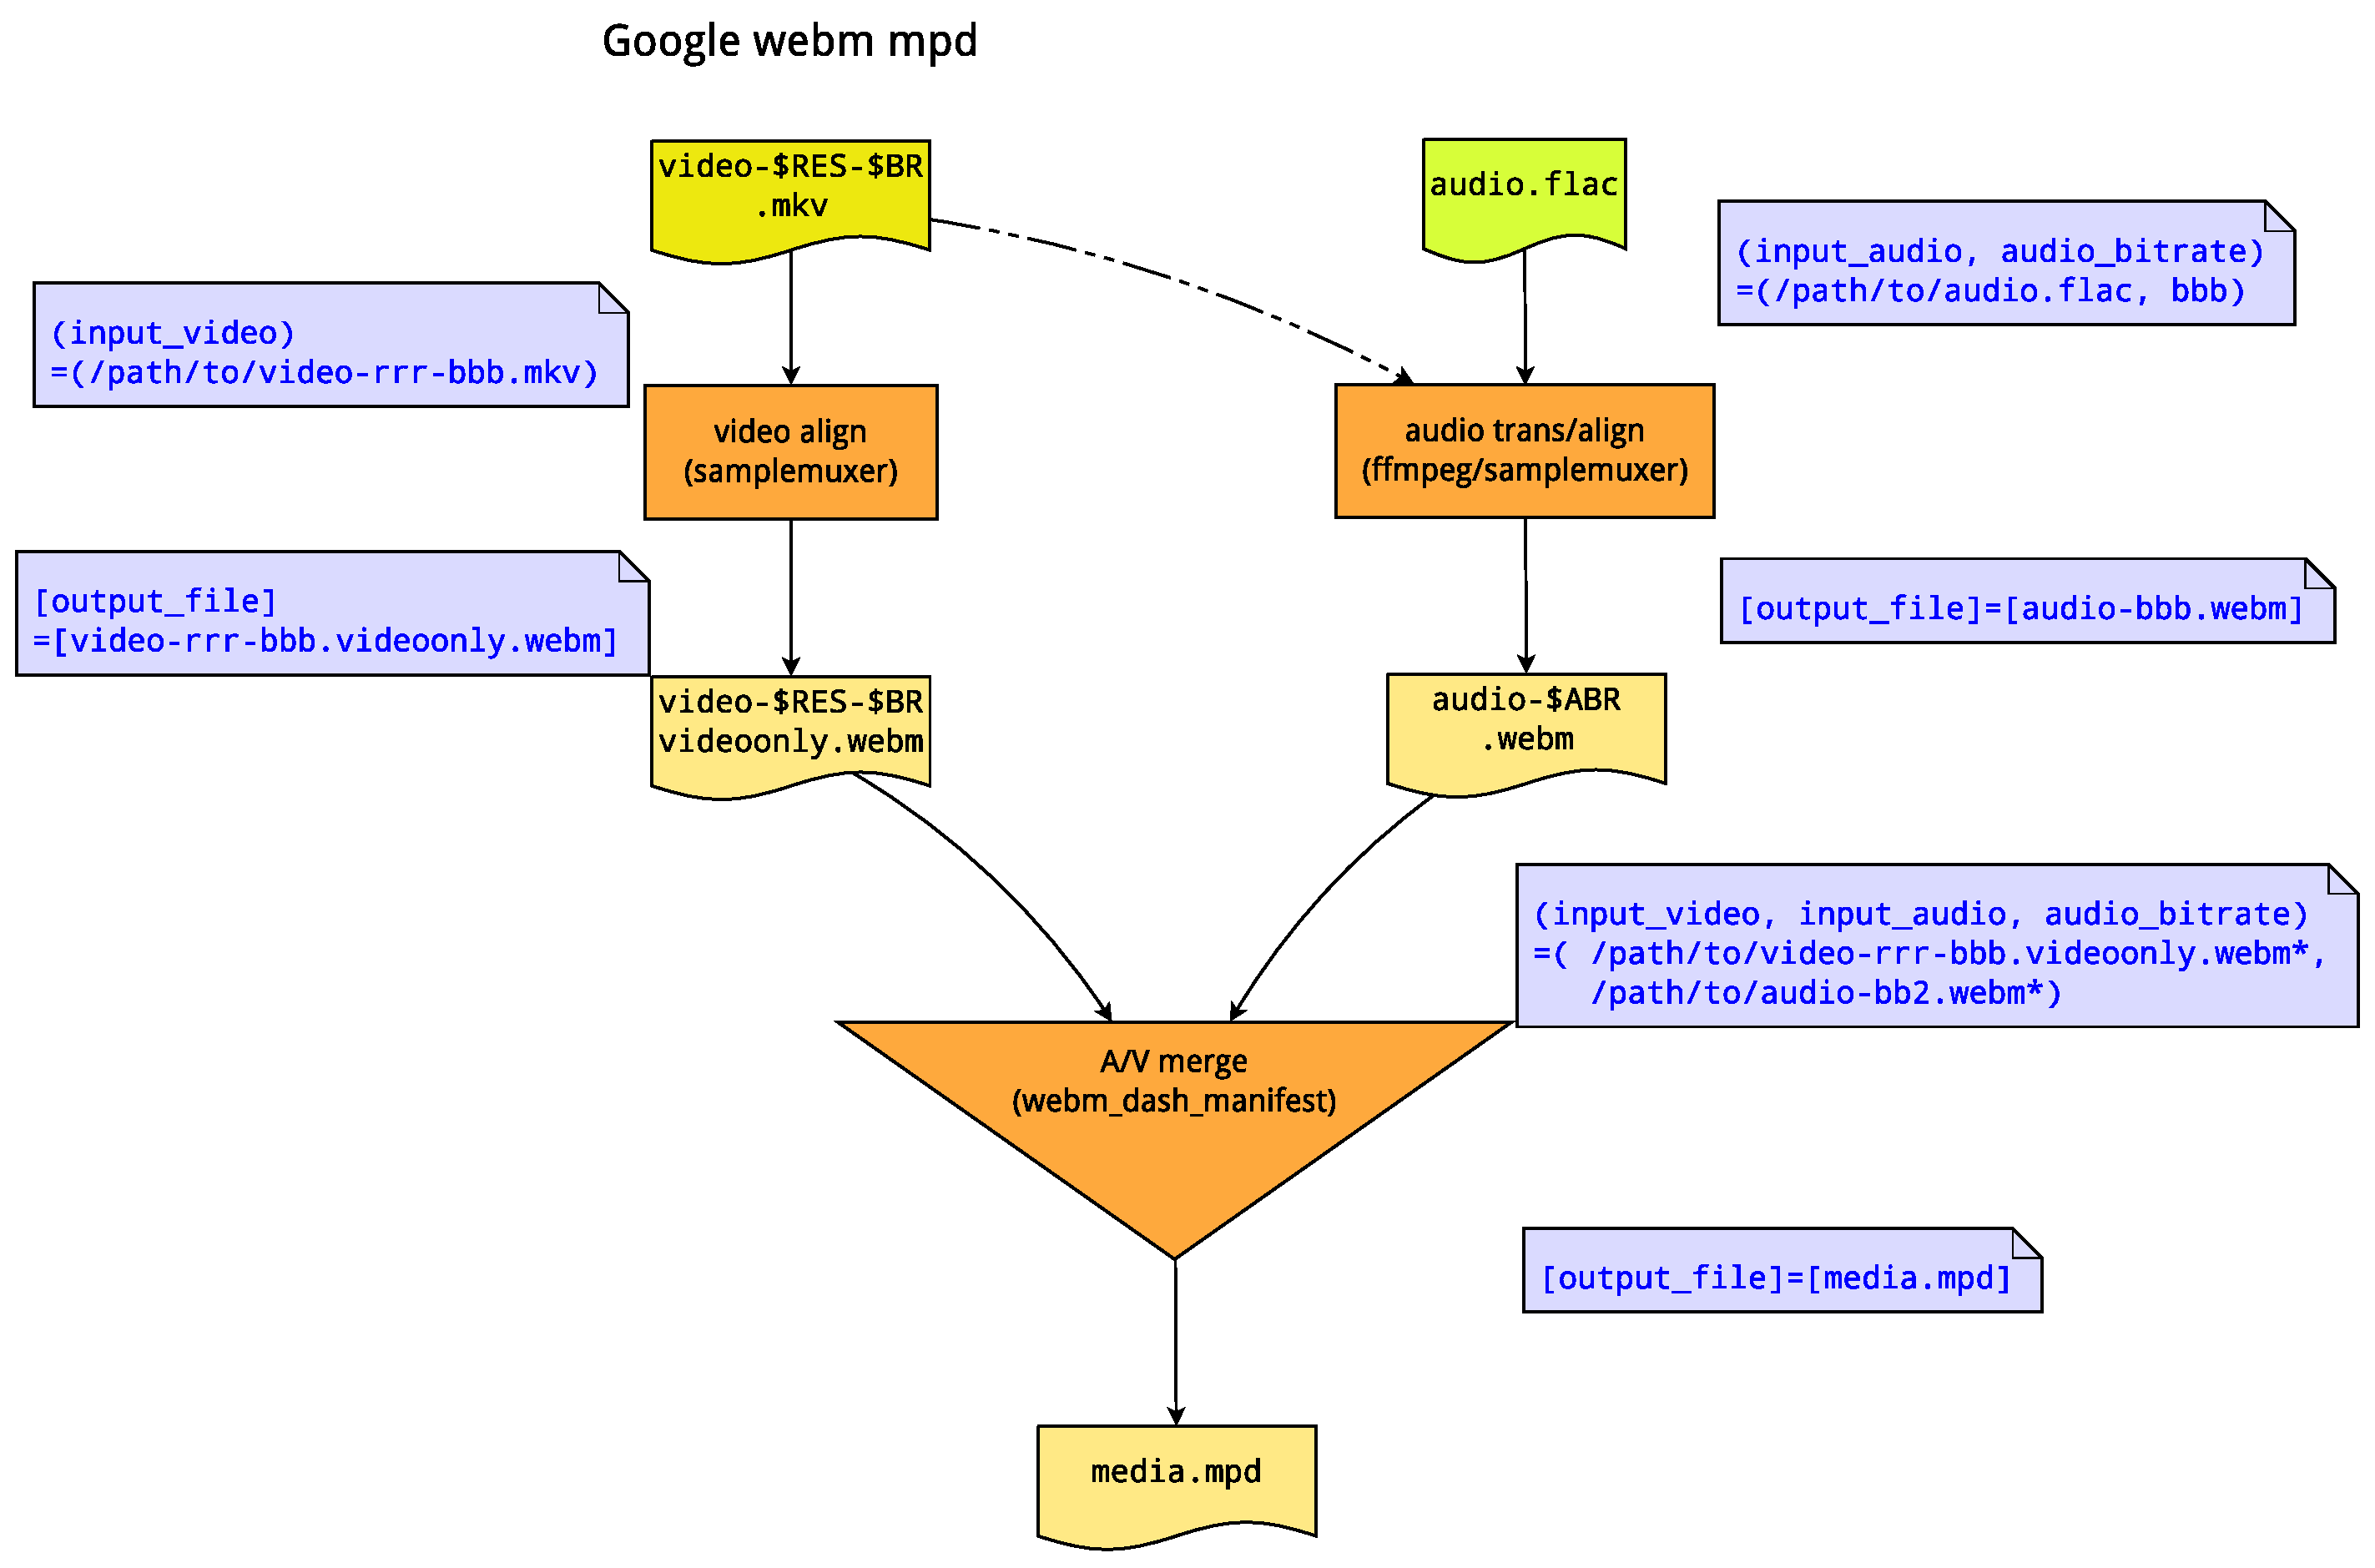
\includegraphics[width=0.9\textwidth]{figures-appconv2dash/flowchart-1-googletoolmpd.eps}
  \caption{Data flow for dashlize by google's tools.}\label{fig:googletoolmpd}
\end{figure}

\begin{lstlisting}[language=bash]
# video transcode
ffmpeg -i video-rrr-bbb.mkv \
    -vcodec libvpx -vb 3800k -s 1920x1080 \
    -keyint_min 150 -g 150 -sc_threshold 0 \
    -an -y video-rrr-bbb.videoonlytmp.mkv
# video align
samplemuxer -i video-rrr-bbb.videoonlytmp.mkv -o video-rrr-bbb.videoonly.mkv

# audio transcode
ffmpeg -i audio.flac -vn -acodec libvorbis -ab 256k -y audio-256k.tmp.webm
# audio align
samplemuxer -i audio-256k.tmp.webm -o audio-256k.webm \
    -output_cues 1 \
    -cues_on_audio_track 1 \
    -max_cluster_duration 5 \
    -audio_track_number 2
\end{lstlisting}

  \item {GPAC MP4Box (mp4)}

MP4Box 会分解文件,生成 mpd 配置文件,参见 \ref{fig:mp4boxmpd}

\begin{figure}\centering
  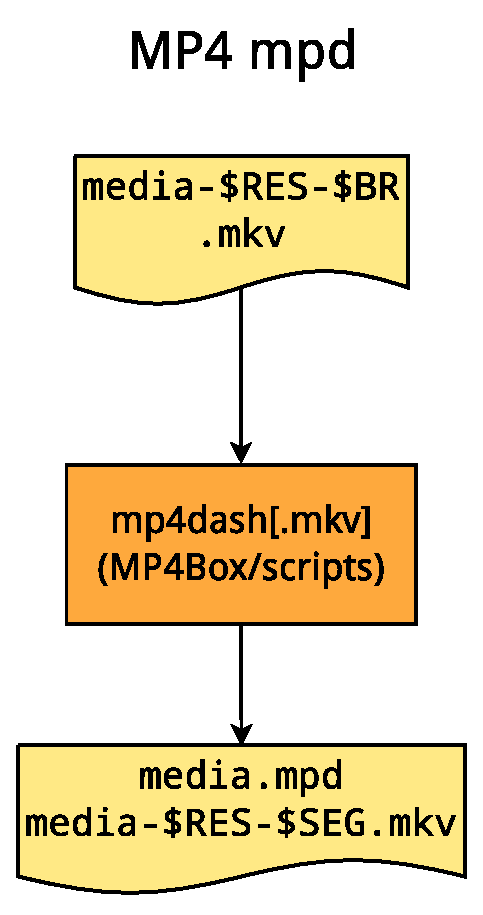
\includegraphics[width=0.3\textwidth]{figures-appconv2dash/flowchart-1-mp4boxmpd.eps}
  \caption{Data flow for dashlize by mp4box.}\label{fig:mp4boxmpd}
\end{figure}

参考命令行:
\begin{lstlisting}[language=bash]
SEGSEC=6
MP4Box -url-template -rap -frag $((500 * ${SEGSEC})) -dash $((1000 * ${SEGSEC})) -segment-name "prefix" "media-rrr-bbb.mkv"
\end{lstlisting}


  \item {dash.js (webm)}


dash.js 的是一个 Python 脚本,参见 \ref{fig:dashjsmpd}.

\begin{figure}\centering
  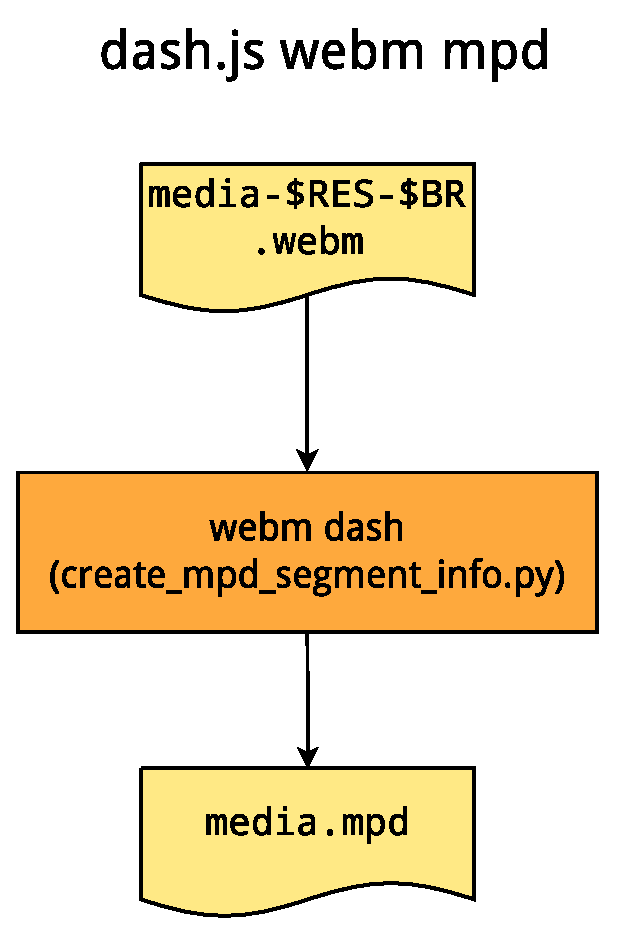
\includegraphics[width=0.3\textwidth]{figures-appconv2dash/flowchart-1-dashjsmpd.eps}
  \caption{Data flow for dashlize by dash.js.}\label{fig:dashjsmpd}
\end{figure}


参考命令行:
\begin{lstlisting}[language=bash]
SEGSEC=6
python dash-js-git/create_mpd_segment_info.py "media-rrr-bbb.webm" ${SEGSEC} $((${SEGSEC} * 2)) "" >> "media.mpd"
\end{lstlisting}

\end{enumerate}


\subsection{Emulation}

TODO






\section{Low Level Design}

Hadoop 中 streaming 模式下区分 key/value 的分节符缺省是 TAB;
也可以通过 \texttt{-D stream.map.output.field.separator=} 来设置。

\begin{itemize}
  \item \texttt{-D stream.map.output.field.separator} -- 设置 map 的输出中 key 和 value 的分隔符
  \item \texttt{-D stream.num.map.output.key.fields} -- 设置 map 的输出中区分 key部分 和 value部分 的分隔符的位置
  \item \texttt{-D map.output.key.field.separator} -- 设置 map 输出中 key 的子分割符
  \item \texttt{-D num.key.fields.for.partition} -- key 按照子分割符切割后,用于分桶 子key 所占的列数
        (使用 \texttt{-partitioner org.apache.hadoop.mapred.lib.KeyFieldBasedPartitioner} )
  \item \texttt{-D stream.reduce.output.field.separator} -- 设置 reduce 输出中 key 和 value 的分隔符
  \item \texttt{-D stream.num.reduce.output.key.fields} -- 设置 reduce 输出中 key部分 和 value部分 的分隔符的位置
\end{itemize}


\subsection{The Transcoding Module}

提供文件转码的功能,将无损视频和音频转换为指定解析度和比特率的多媒体文件和DASH .mpd 文件。

\textbf{问题}

\begin{itemize}
  \item \texttt{ffmpeg -f segment} 分解的文件块不是等 frame 个数,需要在最后附上各个分块的frame个数!
  \item 简化对用户接口。需要用户提供的参数可以缩减到:
    \begin{itemize}
      \item 视频文件类型(图片,视频)和路径
      \item 音频文件
      \item 分片大小
      \item 帧率(图片)
      \item 转码 分辨率-比特率 对(列表)
      \item 视频 matric 屏幕大小列表
    \end{itemize}
  如何设计接口可以让这些参数传递到下级?例如,转码才要用到的 分辨率-比特率 对(列表) 信息。
  针对不同视频比特率的对应的音频比特率如何获取?
  \item 其中音频文件是在任务的中间使用,可以通过配置文件设置,但这样会和用户输入``脱节'',输入参数和视频分开了,
  不容易管理使用。所以,将音频输入文件信息和视频输入信息放在一起输入,这样,程序需要一直传递音频信息直到所需要的地方。

  如果用户处理的时候,可以接受分片文件,包括音频视频分开,则可以不包含音频部分的处理。
\end{itemize}

\subsubsection{Interface of the link pictures/split processing}

使用 hadoop streaming 模式,
输入是含有需要处理的文件的列表。
对于源处理文件是视频单帧图片文件,文件名需要是顺序数字编号的格式;
而要提供 路径名format、分片大小(时间)、起始编号、文件个数、帧率 等五个参数作为输入参数。
输出文件为一系列分片视频文件。

\begin{enumerate}
  \item \textbf{map}
处理:
预先处理文件,
如果是单独视频文件,则分解视频文件,将分块文件名传送到下步做排序后获取各个块的frame大小,计算对应的起始frame编号送给 lossless 处理;
如果是图片,则输出目录下所有文件名,然后通过后面的shuffle排序后分组做无损压缩操作。


输入参数:
\begin{lstlisting}[language=bash]
<type> <audio_file> <video_file_fmt> <segsec> [<fps> <#start> <#files>]
# origpic "/path/to/audio1.flac" "/path/to/film-%05d.png"      6 24 1 1253
# origvid "/path/to/audio2.flac" "/path/to/video-lossless.mkv" 6
\end{lstlisting}


输出:
\begin{lstlisting}[language=bash]
<type> <path_in> <segsec> <audio_file> [<path_out> <fps>]
picgroup   <key> <audio_file> <vid_seg_file_name_out> <segsec> <fps> <frame_start_number>
processvid <key> <audio_file> <vid_seg_file_name_out> <segsec>
# picgroup   "/path/to/film-%05d.png"      "/path/to/audio1.flac" "/path/to/tmp/video-0000000000000000000.lossless.mkv" 6 24 0
# picgroup   "/path/to/film-%05d.png"      "/path/to/audio1.flac" "/path/to/tmp/video-0000000000000000001.lossless.mkv" 6 24 144
# processvid "/path/to/video-lossless.mkv" "/path/to/audio2.flac" "/path/to/tmp/video-0000000000000000001.lossless.mkv" 6
\end{lstlisting}

磁盘上生成对应的图片文件分组目录。

  \item \textbf{reduce}
处理:
将输入转换成无损压缩的分片视频文件。


输入参数:(前4列为key)
\begin{lstlisting}[language=bash]
<type> <path_in> <segsec> <audio_file> [<path_out> <fps>]
picgroup   <key> <audio_file> <vid_seg_file_name_out> <segsec> <fps> <frame_start_number>
processvid <key> <audio_file> <vid_seg_file_name_out> <segsec>
# picgroup   "/path/to/film-%05d.png"      "/path/to/audio1.flac" "/path/to/tmp/video-0000000000000000000.lossless.mkv" 6 24 0
# picgroup   "/path/to/film-%05d.png"      "/path/to/audio1.flac" "/path/to/tmp/video-0000000000000000001.lossless.mkv" 6 24 144
# processvid "/path/to/video-lossless.mkv" "/path/to/audio2.flac" "/path/to/tmp/video-0000000000000000001.lossless.mkv" 6
\end{lstlisting}

输出:
\begin{lstlisting}[language=bash]
<type> <serial#> <video_file> <resolution> <video_bps> <audio_file> <audio_bps>
# lossless 0 "/path/to/tmp/video-0000000000000000000.lossless.mkv"  320x180   315k "/path/to/audio1.flac" 64k
# lossless 0 "/path/to/tmp/video-0000000000000000000.lossless.mkv"  640x360   705k "/path/to/audio1.flac" 64k
# lossless 0 "/path/to/tmp/video-0000000000000000000.lossless.mkv"  853x480  1200k "/path/to/audio1.flac" 192k
# lossless 0 "/path/to/tmp/video-0000000000000000000.lossless.mkv" 1280x720  3200k "/path/to/audio1.flac" 256k
# lossless 0 "/path/to/tmp/video-0000000000000000000.lossless.mkv" 1920x1080 4200k "/path/to/audio1.flac" 256k
# lossless 144 "/path/to/tmp/video-0000000000000000001.lossless.mkv"  320x180   315k "/path/to/audio1.flac" 64k
\end{lstlisting}

磁盘上生成对应的视频分片文件。

视频解析度比特率和音频比特率列表从全局设置文件中读出。
\end{enumerate}


\subsubsection{Interface of the transcoding processing}

转码、串接视频、合并音频。

\begin{enumerate}
  \item \textbf{map}

处理:
将输入无损压缩的分片视频文件 转码成指定的分辨率-比特率 的视频文件。


输入参数:
\begin{lstlisting}[language=bash]
<type> <seq_frame> <video_file> <resolution> <video_bps> <audio_file> <audio_bps>
# lossless 0 "/path/to/tmp/video-0000000000000000000.lossless.mkv"  320x180 315k "/path/to/audio1.flac" 64k
# lossless 144 "/path/to/tmp/video-0000000000000000001.lossless.mkv"  320x180 315k "/path/to/audio1.flac" 64k
\end{lstlisting}

输出:(前2列为关键key,第3列作为排序key的一部分)
\begin{lstlisting}[language=bash]
concat  <video_destination> <transcode_file> <audio_file> <audio_bitrate>
# concat "/path/to/video-320x180-315k.mkv" "/path/to/tmp/video-320x180-315k-0000000000000000000.mkv" "/path/to/audio1.flac" 64k
# concat "/path/to/video-320x180-315k.mkv" "/path/to/tmp/video-320x180-315k-0000000000000000001.mkv" "/path/to/audio1.flac" 64k
\end{lstlisting}

\begin{lstlisting}[language=bash]
metricsv <transcode_file> <mmetrics_destination> <origin_file> <start_frame_number> <screen_resolution>
# metricsv "/path/to/video-320x180-315k.metricsv" "/path/to/tmp/video-320x180-315k-0000000000000000000.mkv" "/path/to/tmp/video-lossless-0000000000000000000.mkv" 0 1280x720
# metricsv "/path/to/video-320x180-315k.metricsv" "/path/to/tmp/video-320x180-315k-0000000000000000001.mkv" "/path/to/tmp/video-lossless-0000000000000000001.mkv" 144 1280x720
\end{lstlisting}

如果输出是 webm格式文件的化:(前3列为key,因为需要分布式处理,key越散越好)
\begin{lstlisting}[language=bash]
audioenc <transcode_file> <origin_file> <audio_bitrate> <mpd_destination>
# audioenc "/path/to/audio-256k.webm" "/path/to/audio.flac" 256k "/path/to/video.gwebm.mpd"
\end{lstlisting}


磁盘上生成对应的视频文件。

concat 类型的 resolution 和 bitrate 是用于 reduce 来做合并操作, 输出的 audio\_bitrate 是给下步做参数用。

下面的reduce处理, concat 主要是集合文件,所以必须以文件名排序(第3列),同时以 destination 为聚合文件名,
所以指定前3列为key,而key 的 partition 为前2列。Hadoop 中的表示是:

\begin{lstlisting}[language=bash]
    -D stream.num.map.output.key.fields=3 \
    -D num.key.fields.for.partition=2 \
\end{lstlisting}

metrics 的记录为了能够打乱顺序(以便负载均衡),原有的 type,destination,trans 被设置为 type,trans,destination。

  \item \textbf{reduce -- concat}

处理:
针对 concat 类型的数据,在所有数据收集齐后,做串接成完整视频的操作.

这时,因为需要支持三种不同工具的 DASH 化操作,需要分开完成相关准备工作。
对于MP4Box和dash.js的工具,需要的输入文件是A/V合并后的文件,所以还需等待后满操作完成后再做。

对于 google tools 是需要 A/V分开的 webm(mp4不支持) 文件,所以在串接视频文件后,需要立即进行,所以在这里需要发出
相关请求(dashwebmgmerge)。
另外,因为音频文件需要单独编码,所以在此步之前发出音频编码指令,在本步另外一个函数平级处理,然后同时也输出 dashwebmgmerge,这样下步可以做生成 mpd 文件的操作。

对于其他两种DASH工具,还需要合并音频。

输入参数:(前2列为关键key,第3列作为排序key的一部分)
\begin{lstlisting}[language=bash]
<type> <video_destination> <transcode_file> <audio_file> <audio_bitrate>
# concat "/path/to/video-320x180-315k.mkv" "/path/to/tmp/video-320x180-315k-0000000000000000001.mkv" "/path/to/audio1.flac" 64k
\end{lstlisting}


输出:(前2列为关键key,第3列作为排序key的一部分)
\begin{lstlisting}[language=bash]
dashwebmgmerge <mpd_destination> <mediatype> <transcode_file>
# dashwebmgmerge "/path/to/video.gwebm.mpd" video "/path/to/video-320x180-315k.mkv"
\end{lstlisting}

输出:
\begin{lstlisting}[language=bash]
dashmpd <mpd_destination> <mediatype> <transcode_file>
# dashmpd "/path/to/video.mpd" av "/path/to/video-320x180-315k.mkv"
\end{lstlisting}

磁盘上生成对应的视频文件。

  \item \textbf{reduce -- metricsv}

处理:

使用 mediamatrics 的 \texttt{-b <start\_frame\_number>} 设置各个分块的起始 frame 号。

输入参数:(前3列为key,因为需要分布式处理,key越散越好)
\begin{lstlisting}[language=bash]
metricsv <mmetrics_destination> <transcode_file> <origin_file> <start_frame_number> <screen_resolution>
# metricsv "/path/to/video-320x180-315k.metricsv" "/path/to/tmp/video-320x180-315k-0000000000000000000.mkv" "/path/to/tmp/video-lossless-0000000000000000000.mkv" 0 1280x720
# metricsv "/path/to/video-320x180-315k.metricsv" "/path/to/tmp/video-320x180-315k-0000000000000000001.mkv" "/path/to/tmp/video-lossless-0000000000000000001.mkv" 144 1280x720
\end{lstlisting}


输出:
\begin{lstlisting}[language=bash]
metricsconcat <mmetrics_destination> <mediatype> <mmetrics_file>
# metricsvconcat "/path/to/video-320x180-315k.metricsv" txt "/path/to/tmp/video-320x180-315k-0000000000000000000.1920x1080.metricsv"
# metricsvconcat "/path/to/video-320x180-315k.metricsv" txt "/path/to/tmp/video-320x180-315k-0000000000000000001.1920x1080.metricsv"
\end{lstlisting}

磁盘上生成对应的视频文件、分片.metricsvideo 文件。

该文件是属于分片视频文件的,下一步需要在所有数据收集完后,进行合并。


  \item \textbf{reduce -- audioenc}

处理:
对音频做编码处理。


输入参数:(前3列为key,因为需要分布式处理,key越散越好)
\begin{lstlisting}[language=bash]
audioenc <transcode_file> <origin_file> <mpd_destination> <audio_bitrate>
# audioenc "/path/to/audio-256k.webm" "/path/to/audio.flac" "/path/to/video.gwebm.mpd" 256k
\end{lstlisting}


输出:(前2列为关键key,第3列作为排序key的一部分)
\begin{lstlisting}[language=bash]
dashwebmgmerge <mpd_destination> <mediatype> <transcode_file>
# dashwebmgmerge "/path/to/video.mpd" audio "/path/to/audio-256k.webm"
\end{lstlisting}

磁盘上生成对应的音频文件。

\end{enumerate}



\subsubsection{Interface of the metrics merging processing}
将 .metricsvideo 文件合并。

指定 reducer 个数为文件个数?


\begin{enumerate}
  \item \textbf{map}
NONE


  \item \textbf{reduce -- metricsvconcat}
处理:

输入参数:(前2列为关键key,第3,4列作为排序key的一部分)
\begin{lstlisting}[language=bash]
metricsvconcat <mmetrics_destination> <mediatype> <mmetrics_file>
# metricsvconcat "/path/to/video-320x180-315k.metricsvideo" txt "/path/to/tmp/video-320x180-315k-0000000000000000000.1920x1080.metricsvideo"
\end{lstlisting}

输出:
/path/to/video-320x180-315k.metricsvideo

磁盘上生成对应合并了的 \texttt{.metricsvideo} 文件。

这里是聚合所有文件,所以文件需要排序(前2列),聚合文件为第1列,所以设置:

\begin{lstlisting}[language=bash]
    -D stream.num.map.output.key.fields=2 \
    -D num.key.fields.for.partition=1 \
\end{lstlisting}




  \item \textbf{reduce -- dashwebmgmerge}
处理:
使用 google tools 的dash工具处理。
需要合并同样 destination 的视频/音频文件。


输入参数:(前2列为关键key,第3,4列作为排序key的一部分)
\begin{lstlisting}[language=bash]
dashwebmgmerge <mpd_destination> <mediatype> <transcode_file>
# dashwebmgmerge "/path/to/video.mpd" video "/path/to/video-320x180-315k.mkv"
\end{lstlisting}

输出:

\texttt{.mpd} 文件。



  \item \textbf{reduce -- dashmpd}
处理:
使用 dash mpd 工具处理。这里可以使用 MP4Box 和 dash.js 的。

输入参数:(前2列为关键key,第3,4列作为排序key的一部分)
\begin{lstlisting}[language=bash]
dashmpd <mpd_destination> <mediatype> <transcode_file>
# dashmpd "/path/to/video.mpd" av "/path/to/video-320x180-315k.mkv"
\end{lstlisting}

输出:

\texttt{.mp4box.mpd},\texttt{.dashjs.mpd} 文件(以及 dash 分片文件).


\end{enumerate}



\subsection{Simulation Emulation}
TBD

\subsection{Data Analysis}
TBD











\section{Implementation}

\subsection{The structure of the working directory}

\begin{itemize}
  \item \texttt{etc}: 一些和系统相关的配置
    \begin{itemize}
      \item \texttt{transcode.conf} 文件转码的一些配置,包括解析度,比特率、转码格式(x264,webm)等。
    \end{itemize}
  \item \texttt{bin}: 编译好的运行程序
  \item \texttt{lib}: 程序依赖库
  \item \texttt{data}: 使用的数据/结果
    \begin{itemize}
      \item \texttt{input}: 原始输入数据
      \item \texttt{output}: 输出数据/结果
      \item \texttt{buffer}: 中间结果
        \begin{itemize}
          \item \texttt{hdfs}: hadoop HDFS 使用的目录(如果有)
        \end{itemize}
  \end{itemize}
\end{itemize}


\subsection{Speed}


\subsubsection{测试方法}

为了对比单机和分布式速度上的提速,可以分别测试在单线程和多线程配置下的速度。

\begin{itemize}
  \item 单节点上单进程、ffmpeg 配置为单线程
  \item 单节点上单进程、ffmpeg 配置为多线程(3线程)
  \item 单节点上多进程(3进程)、ffmpeg 配置为单线程
  \item 单节点上多进程(3进程)、ffmpeg 配置为多线程(3线程)
  
\end{itemize}





以下是
在 i5-3360M 2核,4线程,16G RAM 机器上;
内存消耗小于4G.

\subsubsection{test 1}
webm

HDFF\_TRANSCODE\_RESOLUTIONS=320x180+315k+64k,640x360+500k+64k

HDFF\_SCREEN\_RESOLUTIONS=320x180


sintel trailer, png files, trancode, mediametric
\begin{lstlisting}[language=bash]
sh1 -- 203
hadoop -- 282
\end{lstlisting}


sintel trailer, 1080p mkv files, trancode, mediametric
\begin{lstlisting}[language=bash]
sh1 -- 241
hadoop -- 318
\end{lstlisting}


sintel trailer, png files + 1080p mkv file, trancode, mediametric
\begin{lstlisting}[language=bash]
sh1 -- 424
hadoop -- 516
\end{lstlisting}


\subsubsection{test 2}
webm

HDFF\_TRANSCODE\_RESOLUTIONS=320x180+315k+64k,640x360+500k+64k

HDFF\_SCREEN\_RESOLUTIONS=320x180


sintel trailer, png files
\begin{lstlisting}[language=bash]
1 process, 1 thread
[run-sh1.sh] Cost time: total=326 seconds
    stage1=57(m=0,r=57) seconds
    stage2=268(m=163,r=105) seconds
    stage3=1(m=0,r=1) seconds


1 process, 3 threads
[run-sh1.sh] Cost time: total=288 seconds
    stage1=51(m=1,r=50) seconds
    stage2=237(m=117,r=120) seconds
    stage3=0(m=0,r=0) seconds


3 processes, 1 threads
[run-sh1.sh] Cost time: total=211 seconds
    stage1=41(m=0,r=41) seconds
    stage2=169(m=90,r=79) seconds
    stage3=1(m=0,r=1) seconds


3 processes, 3 threads
[run-sh1.sh] Cost time: total=195 seconds
    stage1=42(m=1,r=41) seconds
    stage2=152(m=78,r=74) seconds
    stage3=1(m=0,r=1) seconds


auto: 3 processes, 2 threads
[run-sh1.sh] Cost time: total=226 seconds
    stage1=48(m=1,r=47) seconds
    stage2=177(m=89,r=88) seconds
    stage3=1(m=0,r=1) seconds
[run-sh1.sh] Cost time: total=211 seconds
    stage1=40(m=1,r=39) seconds
    stage2=171(m=92,r=79) seconds
    stage3=0(m=0,r=0) seconds
[run-sh1.sh] Cost time: total=229 seconds
    stage1=45(m=1,r=44) seconds
    stage2=183(m=96,r=87) seconds
    stage3=1(m=0,r=1) seconds


4 processes, 4 threads
[run-sh1.sh] Cost time: total=225 seconds
    stage1=47(m=1,r=46) seconds
    stage2=177(m=90,r=87) seconds
    stage3=1(m=0,r=1) seconds

# pic
palmetto, user, 21 processes, 7 threads
from /newscratch
[run-sh1.sh] config:
    HDFF_NUM_CLONE=21
    OPTIONS_FFM_GLOBAL= -threads 7
[run-sh1.sh] Cost time: total=870 seconds
    stage1=828(m=312,r=516) seconds
    stage2=41(m=17,r=24) seconds
    stage3=1(m=0,r=1) seconds

from /home
[run-sh1.sh] config:
    HDFF_NUM_CLONE=21
    OPTIONS_FFM_GLOBAL= -threads 7
[run-sh1.sh] Cost time: total=68 seconds
    stage1=37(m=1,r=36) seconds
    stage2=30(m=17,r=13) seconds
    stage3=1(m=0,r=1) seconds


# sintel
[run-sh1.sh] config:
    HDFF_NUM_CLONE=16
    OPTIONS_FFM_GLOBAL= -threads 0
[run-sh1.sh] Cost time: total=157269 seconds
    stage1=12840(m=4307,r=8533) seconds
    stage2=144311(m=4543,r=139678) seconds
    stage3=1(m=1,r=207) seconds


# tear of steel
[run-sh1.sh] config:
    HDFF_NUM_CLONE=16
    OPTIONS_FFM_GLOBAL= -threads 0
[run-sh1.sh] Cost time: total=47255 seconds
    stage1=2177(m=636,r=1541) seconds
    stage2=448833(m=2826,r=42057) seconds
    stage3=1(m=0,r=159) seconds


# BBB, no screen metrics
[run-sh1.sh] config:
    HDFF_NUM_CLONE=16
    OPTIONS_FFM_GLOBAL= -threads 0
[run-sh1.sh] Cost time: total=3912 seconds
    stage1=1995(m=437,r=1558) seconds
    stage2=1902(m=1798,r=104) seconds
    stage3=15(m=0,r=15) seconds

# BBB, with screen metrics
[run-sh1.sh] config:
    HDFF_NUM_CLONE=16
    OPTIONS_FFM_GLOBAL= -threads 0
[run-sh1.sh intercept] Cost time: total=84747 seconds
    stage1=1995(m=437,r=1558) seconds
    stage2=82554(m=1798,r=80756) seconds
    stage3=1(m=0,r=198) seconds


# elephent, with screen metrics
[run-sh1.sh] config:
    HDFF_NUM_CLONE=16
    OPTIONS_FFM_GLOBAL= -threads 0
[run-sh1.sh intercept] Cost time: total=107550 seconds
    stage1=1247(m=295,r=952) seconds
    stage2=106168(m=1775,r=104393) seconds
    stage3=1(m=1,r=134) seconds


\end{lstlisting}





%# -*- coding: utf-8 -*-
% !TeX encoding = UTF-8 Unicode
% !TeX spellcheck = en_US
% !TeX TS-program = xelatex
%~ \XeTeXinputencoding "UTF-8"
% vim:ts=4:sw=4
%
% 以上设定默认使用 XeLaTex 编译,并指定 Unicode 编码,供 TeXShop 自动识别

\chapter{app-wpapw}

\section{High Level Design}



\begin{enumerate}
  \item 使用 flowchart 将处理流程初步理清
  \item 使用 \href{http://www.cascading.org/}{Cascading}/MapReduce 实现系统
  \item 测试
\end{enumerate}


\subsection{介绍}


REF:
\href{https://suprafortix.wordpress.com/tag/rockyou-txt/}{Hashcat Password Cracking, such as no rule and rule crack}
\href{https://hashcat.net/wiki/doku.php?id=cracking_wpawpa2}{hashcat wiki, dic+bruteforce+rule}


\begin{lstlisting}[language=bash]
# command line to crack with dictionary
hashcat -m 2500 for-science-hs.hccap ZD_Tirom_Merger+Trim_8-16_v09d.txt

# with rule
hashcat -m 2500 -r rules/best64.rule for-science-hs.hccap ZD_Tirom_Merger+Trim_8-16_v09d.txt
\end{lstlisting}



\begin{enumerate}
  \item input task:
  convert the input to various actions:
 1. dictionary
 2. brute force (pattern) + rules
 detect how many GPU cards, "hashcat -I"
 use a global variable to store the used card(or left card?)

 for example, ATTXXX, will be consider to run both dic and brute force,
 and brute force is base on the default factory password, which is 10 digital numbers.
 so the software will generate following internal lines:

\begin{lstlisting}[language=bash]
#  <type>, <filename>, <pw type>,   <pw dictionary>
   wifi, test.hs.hccap, dictionary, wordlist1.txt,
   wifi, test.hs.hccap, dictionary, wordlist2.txt,
   wifi, test.hs.hccap, dictionary, wordlist3.txt,
   wifi, test.hs.hccap, dictionary, wordlist4.txt,
   wifi, test.hs.hccap, dictionary, wordlist5.txt,
   wifi, test.hs.hccap, dictionary, wordlist6.txt,

#  <type>, <filename>, <pw type>,   <pw pattern>
   wifi, test.hs.hccap, mask, 0?d?d?d?d?d?d?d?d?d, 
   wifi, test.hs.hccap, mask, 1?d?d?d?d?d?d?d?d?d, 
   wifi, test.hs.hccap, mask, 2?d?d?d?d?d?d?d?d?d, 
   wifi, test.hs.hccap, mask, 3?d?d?d?d?d?d?d?d?d, 
   wifi, test.hs.hccap, mask, 4?d?d?d?d?d?d?d?d?d, 
   wifi, test.hs.hccap, mask, 5?d?d?d?d?d?d?d?d?d, 
   wifi, test.hs.hccap, mask, 6?d?d?d?d?d?d?d?d?d, 
   wifi, test.hs.hccap, mask, 7?d?d?d?d?d?d?d?d?d, 
   wifi, test.hs.hccap, mask, 8?d?d?d?d?d?d?d?d?d, 
   wifi, test.hs.hccap, mask, 9?d?d?d?d?d?d?d?d?d, 

#  <type>, <filename>, <pw type>,   <pw pattern>, <rule>
   wifi, test.hs.hccap, rule, 0?d?d?d?d?d?d?d?d?d, best64
   wifi, test.hs.hccap, rule, 1?d?d?d?d?d?d?d?d?d, best64
   wifi, test.hs.hccap, rule, 2?d?d?d?d?d?d?d?d?d, best64
   wifi, test.hs.hccap, rule, 3?d?d?d?d?d?d?d?d?d, best64
   wifi, test.hs.hccap, rule, 4?d?d?d?d?d?d?d?d?d, best64
   wifi, test.hs.hccap, rule, 5?d?d?d?d?d?d?d?d?d, best64
   wifi, test.hs.hccap, rule, 6?d?d?d?d?d?d?d?d?d, best64
   wifi, test.hs.hccap, rule, 7?d?d?d?d?d?d?d?d?d, best64
   wifi, test.hs.hccap, rule, 8?d?d?d?d?d?d?d?d?d, best64
   wifi, test.hs.hccap, rule, 9?d?d?d?d?d?d?d?d?d, best64
\end{lstlisting}

so the hashcat will run according to the lines, and output lines if the password found:
\begin{lstlisting}[language=bash]
#  <type>, <filename>, <result>,   <password>
   wifi, test.hs.hccap, found, 1234567890
   wifi, test.hs.hccap, notfound,
\end{lstlisting}

 dictionary
 ? support compressed?
 kali default /usr/share/wordlists/
   such as rockyou.txt

  \item the hashcat will run according to the lines generated
\end{enumerate}





the gpu card run the hash code in speed of around 50k,
specifically, it is 77366 H/s for a Tesla K40m,
and 60960 H/s for a NVIDIA GeForce GTX 960M.

we split the pattern to multiple segments,
and also split the dictionary to multiple segments,
so each segment contains same number of words;

the average time for switching tasks would be 2 seconds,
and we want this time is less than 1% of the total time,
so the we want a word/pattern segment involved in computing at least 2/1% =200 seconds,

so the number of word for each segment is 60k * 200 = 12000k
we select 10m as the number of word in the segmen



\subsection{整体结构}
图 \ref{fig:system} 是整个系统的运行框架。

\definecolor{vidtransoriginfile}{HTML}{D7FE39}
\definecolor{vidtranstmpfile}{HTML}{EDE80F}
\definecolor{vidtransfinalfile}{HTML}{FFE985}
\definecolor{vidtransprocess}{HTML}{FEA93E}
\definecolor{vidtransfuncio}{HTML}{DADAFF}
\begin{figure}\centering
  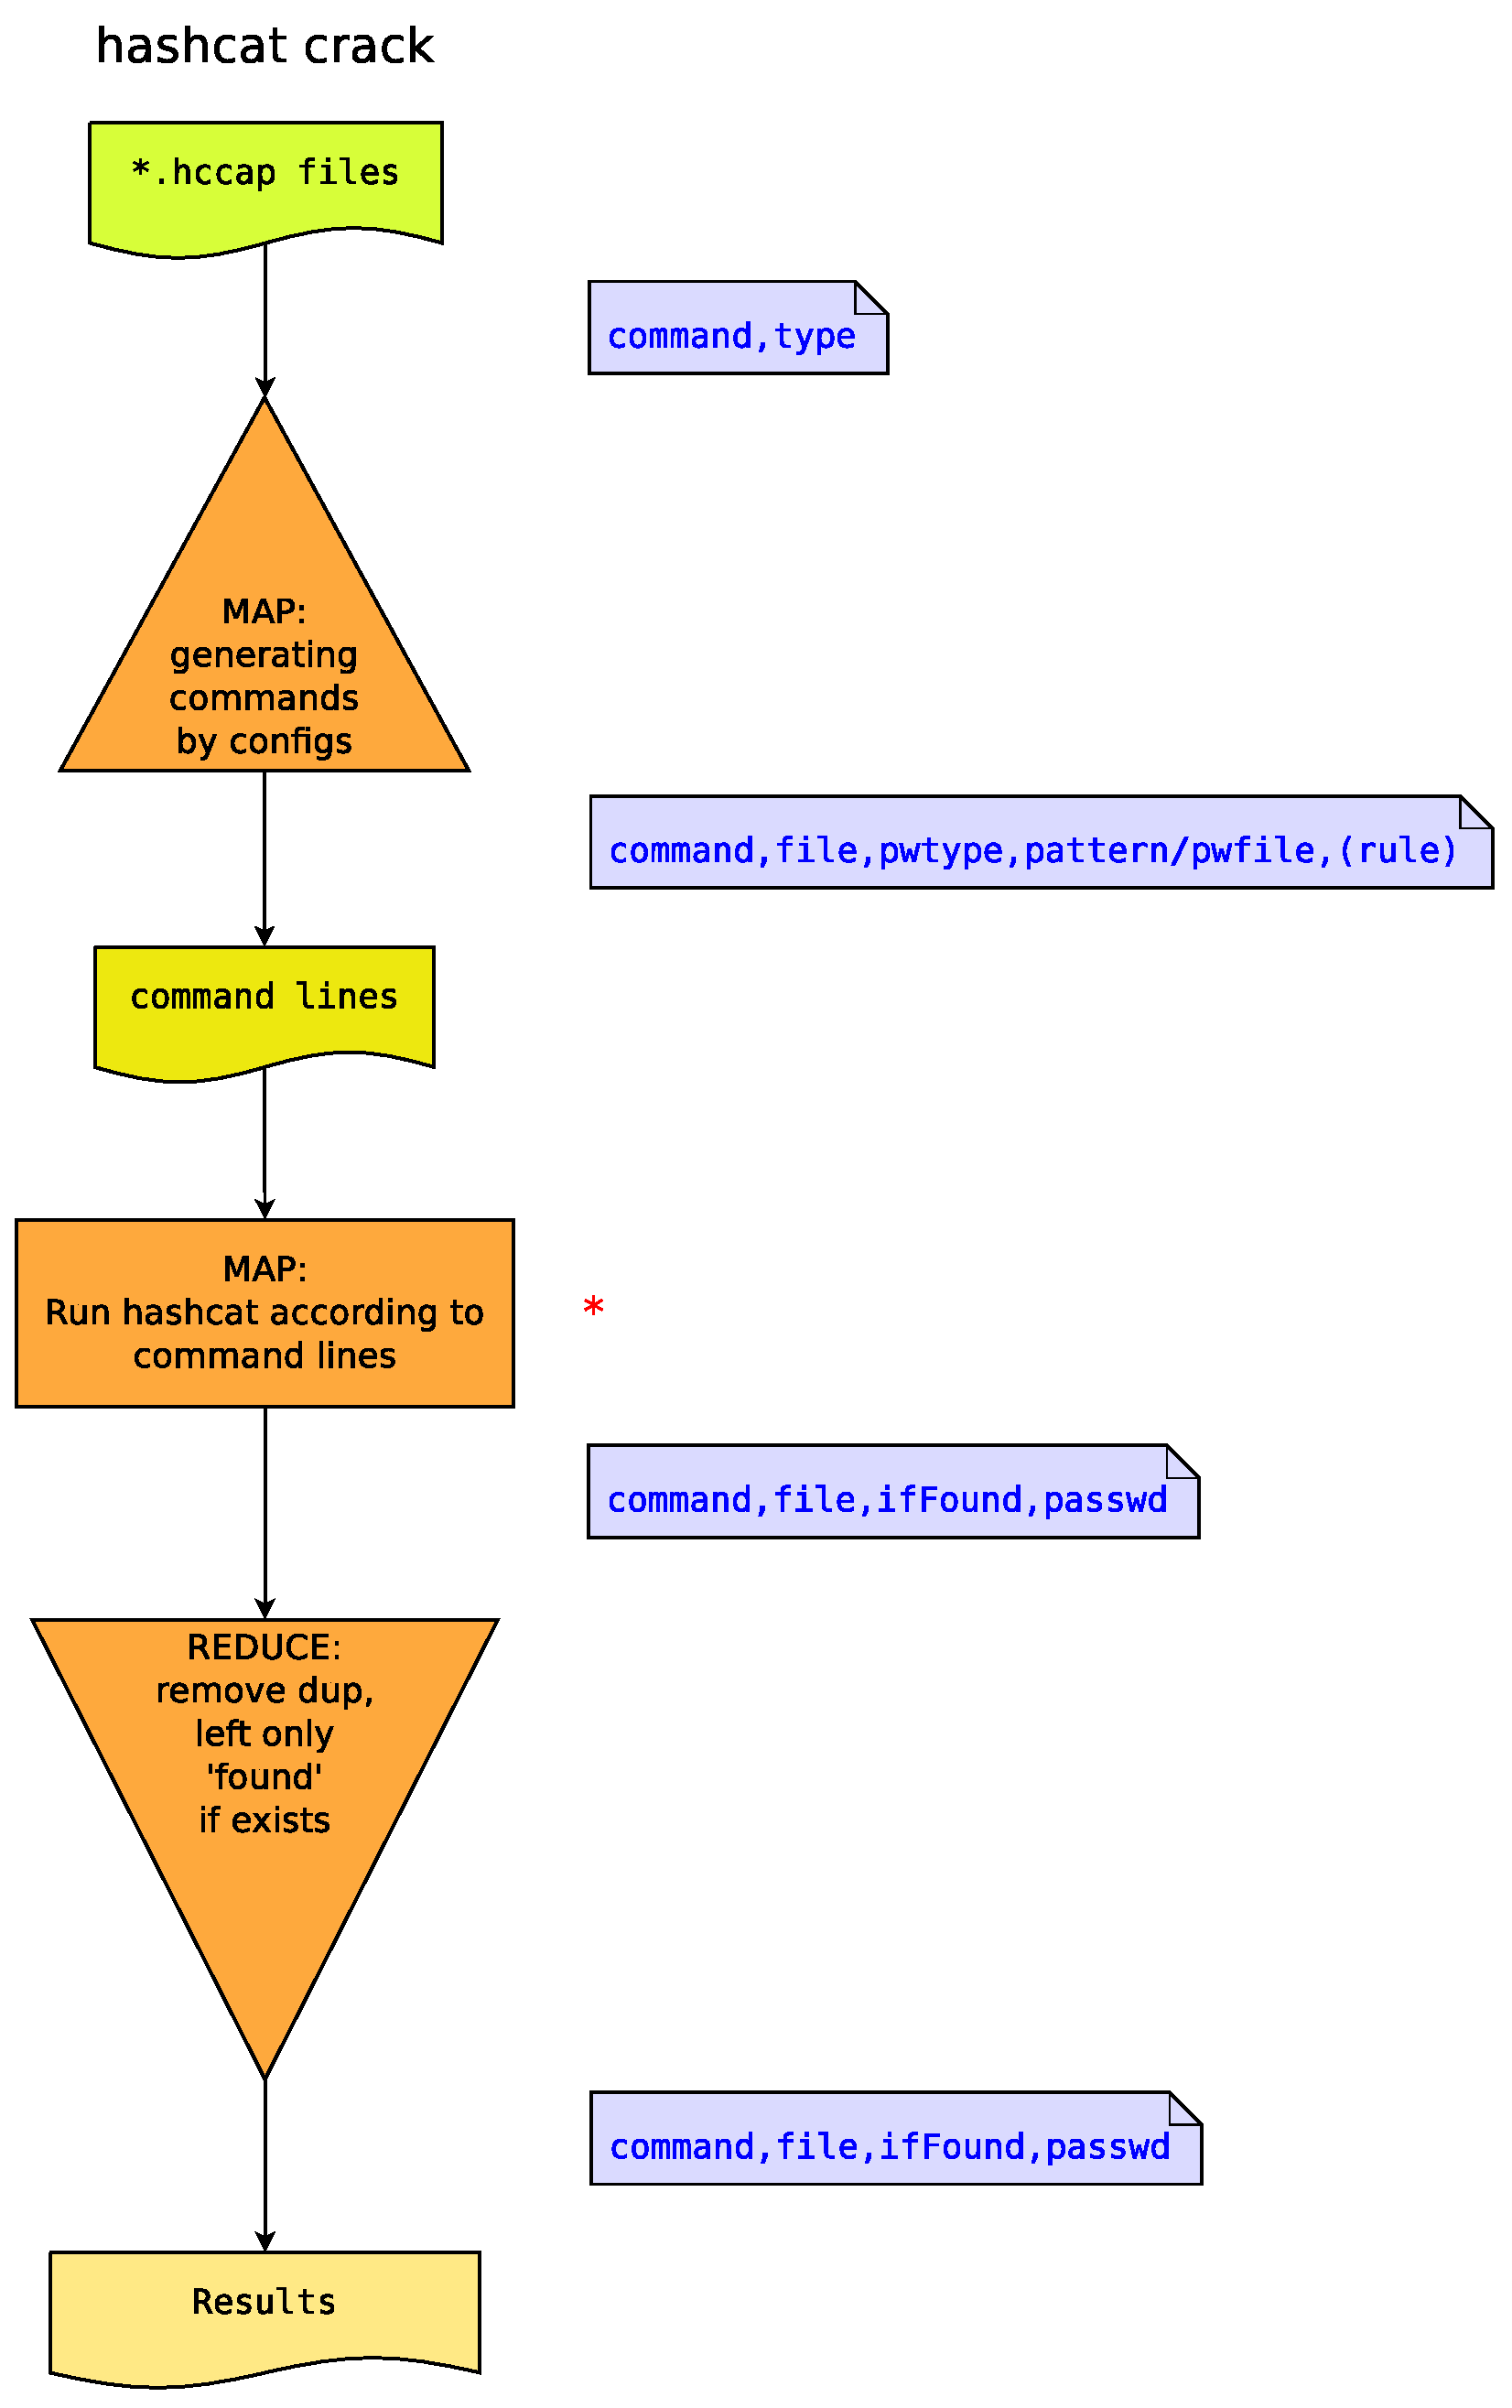
\includegraphics[width=0.5\textwidth]{flowchart-mr-wpapw}
  \caption{The system.
    The text in \fcolorbox{black}{vidtransoriginfile}{this color} is the original input file.
    The text in \fcolorbox{black}{vidtranstmpfile}{this color} is the temp file.
    The text in \fcolorbox{black}{vidtransfinalfile}{this color} is the final output file.
    The text in \fcolorbox{black}{vidtransprocess}{this color} is process block.
    The text in \fcolorbox{black}{vidtransfuncio}{\textcolor[HTML]{0000FF}{this color}} is the input/output of one process block.
The process blocks signed by a \textcolor[HTML]{FF0000}{*} are the blocks cost most of the processing time.
  }\label{fig:system}
\end{figure}



\section{Low Level Design}
TODO


\section{Performance}
TODO

%# -*- coding: utf-8 -*-
% !TeX encoding = UTF-8 Unicode
% !TeX spellcheck = en_US
% !TeX TS-program = xelatex
%~ \XeTeXinputencoding "UTF-8"
% vim:ts=4:sw=4
%
% 以上设定默认使用 XeLaTex 编译,并指定 Unicode 编码,供 TeXShop 自动识别

\chapter{app-ns2}

\section{High Level Design}



\begin{enumerate}
  \item 使用 flowchart 将处理流程初步理清
  \item 使用 \href{http://www.cascading.org/}{Cascading}/MapReduce 实现系统
  \item 测试
\end{enumerate}


\subsection{介绍}

\begin{enumerate}
  \item simulation task:
  generate the NS2 TCL scripts, and run ns2

  \item plotting figures:
  
\end{enumerate}


\subsection{整体结构}
图 \ref{fig:system} 是整个系统的运行框架。

\definecolor{vidtransoriginfile}{HTML}{D7FE39}
\definecolor{vidtranstmpfile}{HTML}{EDE80F}
\definecolor{vidtransfinalfile}{HTML}{FFE985}
\definecolor{vidtransprocess}{HTML}{FEA93E}
\definecolor{vidtransfuncio}{HTML}{DADAFF}
\begin{figure}\centering
  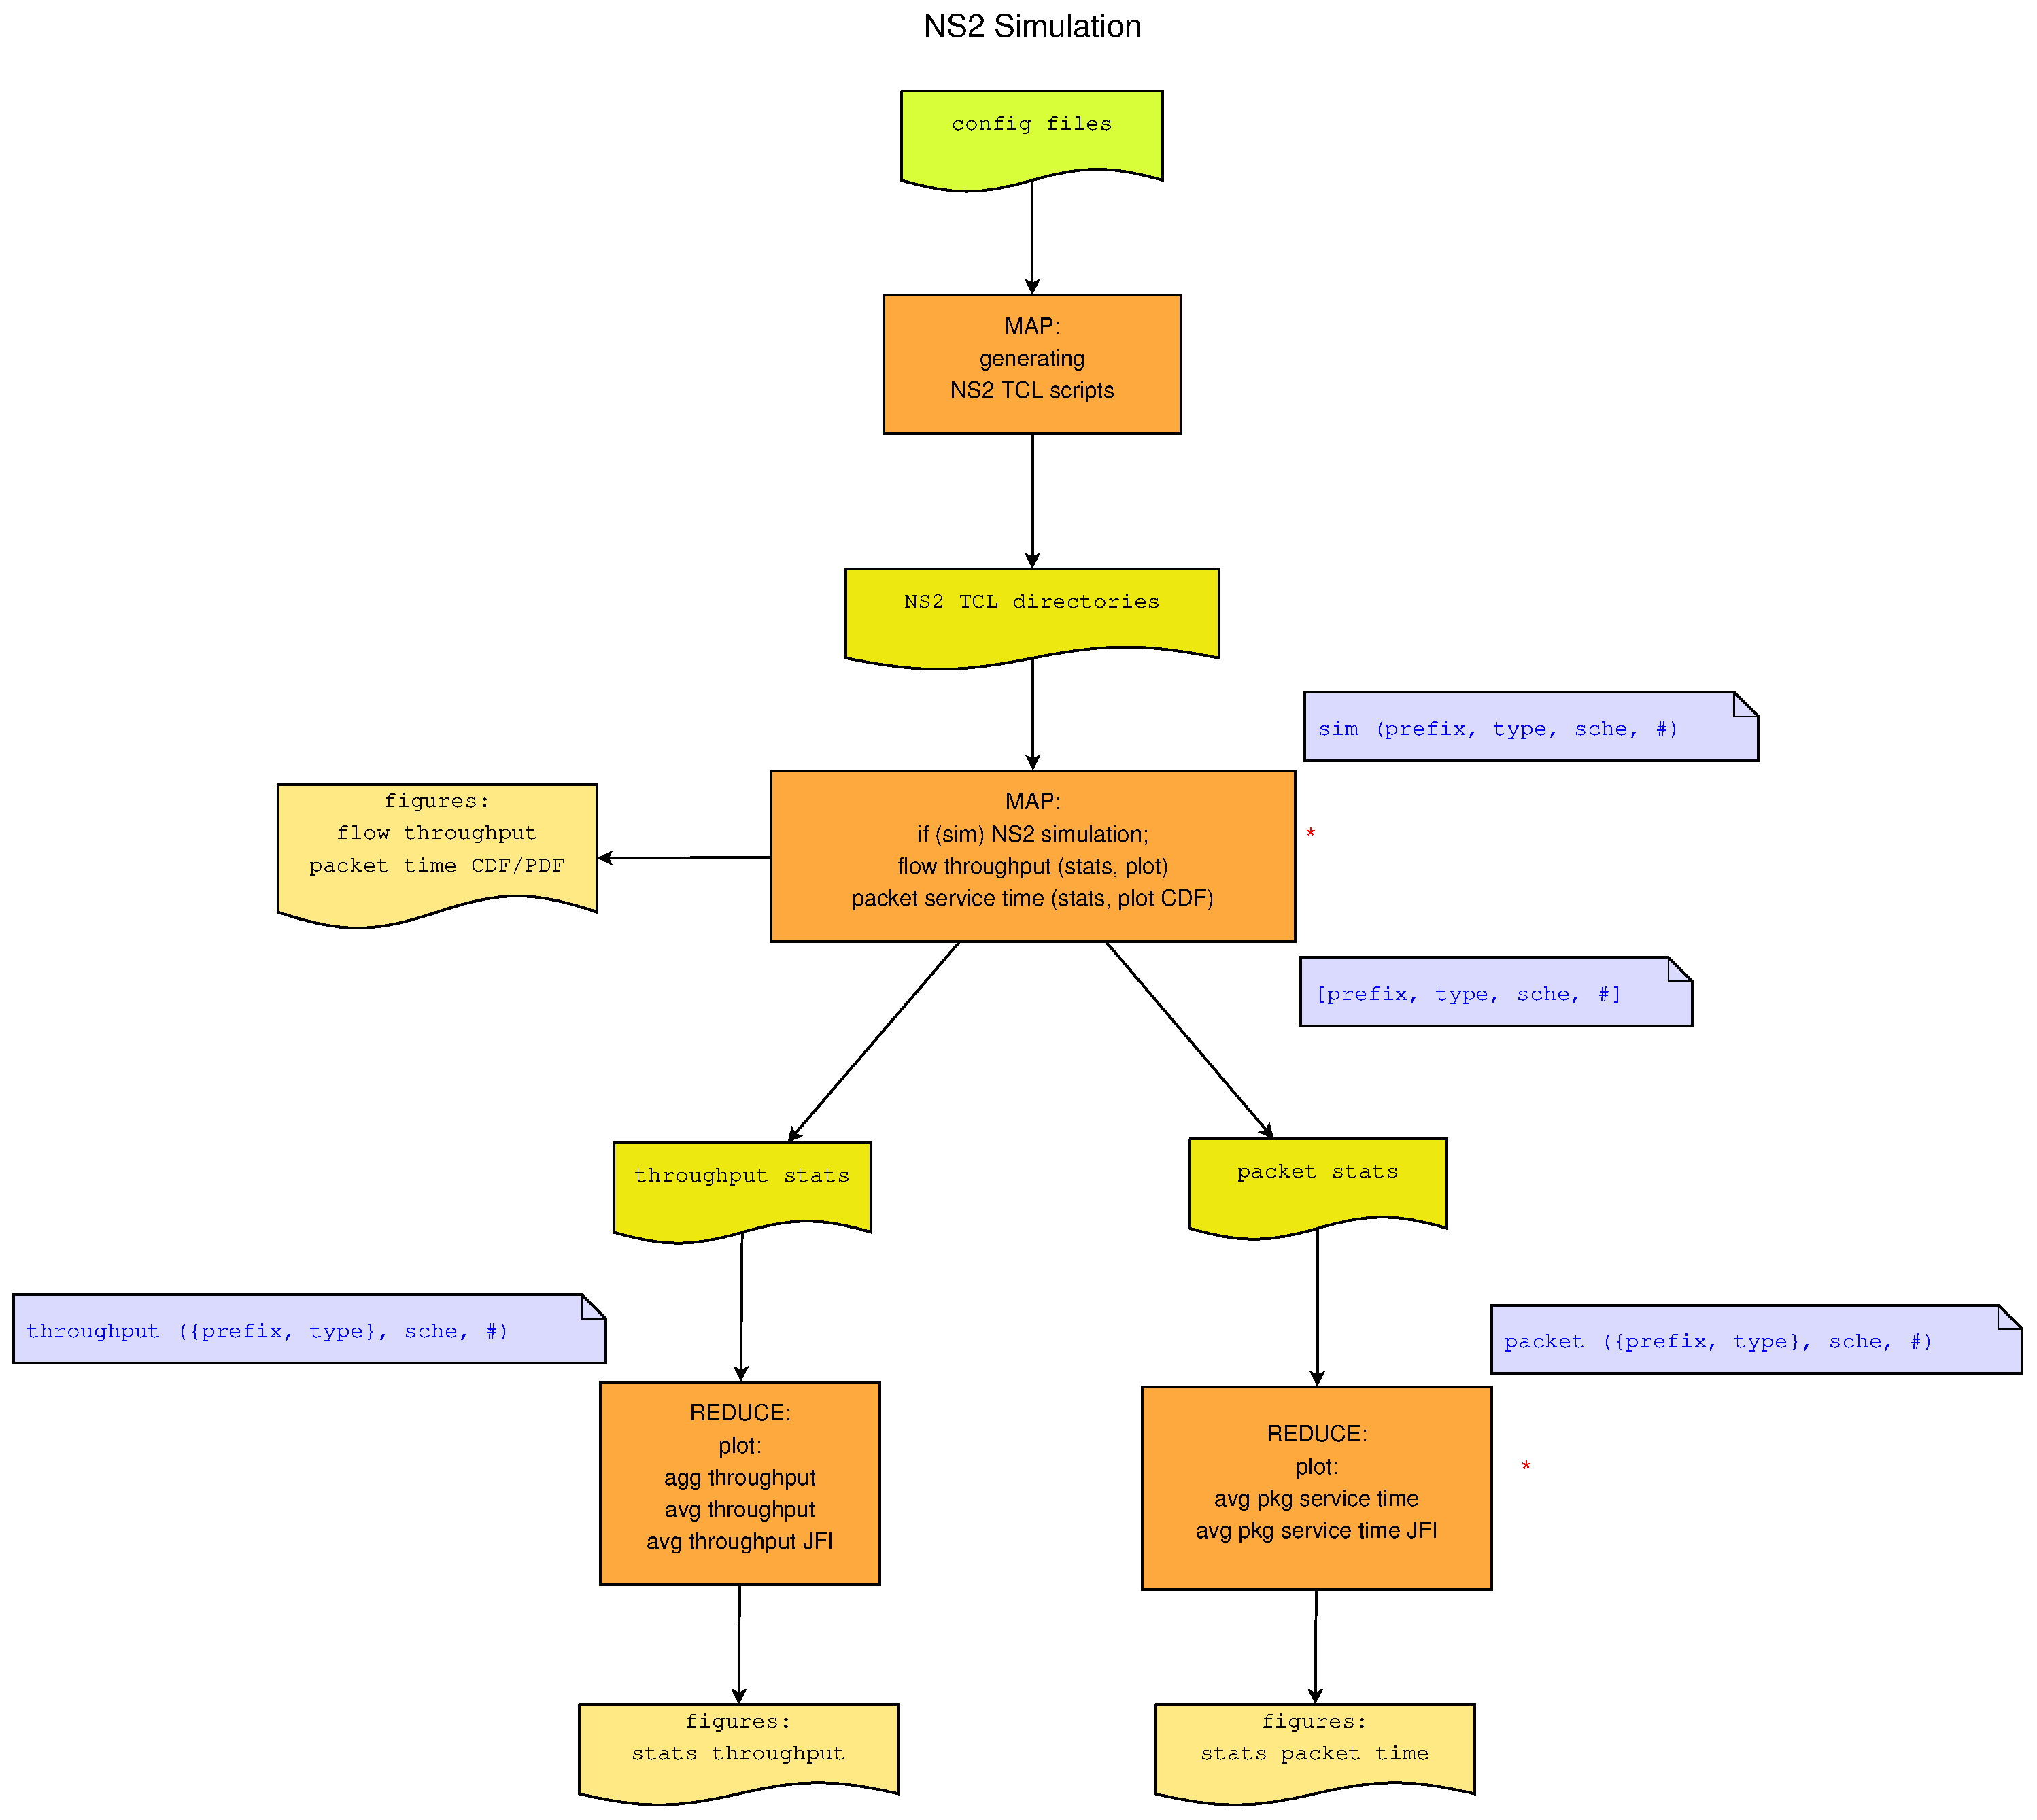
\includegraphics[width=0.9\textwidth]{flowchart-mr-ns2sim}
  \caption{The system.
    The text in \fcolorbox{black}{vidtransoriginfile}{this color} is the original input file.
    The text in \fcolorbox{black}{vidtranstmpfile}{this color} is the temp file.
    The text in \fcolorbox{black}{vidtransfinalfile}{this color} is the final output file.
    The text in \fcolorbox{black}{vidtransprocess}{this color} is process block.
    The text in \fcolorbox{black}{vidtransfuncio}{\textcolor[HTML]{0000FF}{this color}} is the input/output of one process block.
The process blocks signed by a \textcolor[HTML]{FF0000}{*} are the blocks cost most of the processing time.
  }\label{fig:system}
\end{figure}

The packet delay time processing includes:
\begin{itemize}
  \item (Mgn) filter out CMTS management packets and stats
  \item (DS) filter out CMTS--CM flow and stats
  \item (US) filter out CM-CMTS flow and stats
  \item Plot DS CDF/PDF
  \item Plot Managment CDF/PDF
\end{itemize}


\section{Low Level Design}

\subsection{main}


\subsubsection{Interface of the generating configurations}

Use the streaming mode of Map-Reduce.

The input should be the config file list.

\begin{itemize}
  \item \textbf{Map}
Function: generate directories and move and modify TCL scripts for the test.


Input parameters:
\begin{lstlisting}[language=bash]
<command> <config_file>
# config "/path/to/config.sh"
# config "/path/to/config-jjmbase.sh"
\end{lstlisting}


Output:
\begin{lstlisting}[language=bash]
<command> <config_file> <prefix> <type> <scheduler> <number_of_node>
sim <config_file> <prefix> <type> <scheduler> <number_of_node>
# sim "config-xxx.sh" "jjmbase"  "tcp" "PF" 24
\end{lstlisting}

There should exist the directory contains the TCL scripts and data files for the simulation.

\end{itemize}



\subsubsection{Interface of simulation}

This stage will run the simulation base on each directory configuration,
and also generate the related throughput figures.

\begin{itemize}
  \item \textbf{map}
Function: run the simulations.


Input parameters:
\begin{lstlisting}[language=bash]
<command> <config_file> <prefix> <type> <scheduler> <number_of_node>
sim <config_file> <prefix> <type> <scheduler> <number_of_node>
# sim "config-xx.sh" "jjmbase"  "tcp" "PF" 24
\end{lstlisting}


Output:
\begin{lstlisting}[language=bash]
<command> <config_file> <prefix> <type> <flow_type> <scheduler> <number_of_node>
throughput <config_file> <prefix> <type> <flow_type> <scheduler> <number_of_node>
packet <config_file> <prefix> <type> <flow_type> <scheduler> <number_of_node>
# throughput "config-xx.sh" "jjmbase"  "tcp" "tcp" "PF" 24
# packet "config-xx.sh" "jjmbase"  "tcp+has" "tcp" "PF" 24
\end{lstlisting}

The routine should run ns2 and process stats, figures of throughput/packet.




  \item \textbf{reduce}
Function: plot JFI figures


Input: (all of the columns are keys)
\begin{lstlisting}[language=bash]
<command> <config_file> <prefix> <type> <flow_type> <scheduler> <number_of_node>
throughput <config_file> <prefix> <type> <flow_type> <scheduler> <number_of_node>
packet <config_file> <prefix> <type> <flow_type> <scheduler> <number_of_node>
# throughput "config-xx.sh" "jjmbase"  "tcp" "tcp" "PF" 24
# packet "config-xx.sh" "jjmbase"  "tcp+has" "tcp" "PF" 24
\end{lstlisting}

Output: figures

\end{itemize}





\subsection{utils}

We have following program entrances for various execution environments:

\begin{itemize}
  \item \texttt{run-sh1.sh}, run in a single host, to test the basic functions of the software;


    It will call following scripts
    \begin{itemize}
      \item \texttt{e1map.sh}
      \item \texttt{e2map.sh}
      \item \texttt{e2red.sh}
      \item \texttt{e3map.sh}
    \end{itemize}
  \item \texttt{run-hadoop.sh}, setup basic Hadoop environment, copy executable and data to HDFS, call \texttt{mod-share-worker.sh};
    \begin{itemize}
      \item \texttt{mod-share-worker.sh}, the hadoop main script, it will submit various map-reduce tasks for the simulation and data processing;
        \begin{itemize}
          \item \texttt{e1map.sh}
          \item \texttt{e2map.sh}
          \item \texttt{e2red.sh}
          \item \texttt{e3map.sh}
        \end{itemize}
    \end{itemize}

  \item \texttt{run-hadooppbs.sh}, get available HPC resources, setup basic resources info for Hadoop (cores, memory etc.), submit \texttt{mod-hadooppbs-jobmain.sh} to the PBS;

    \begin{itemize}
      \item \texttt{mod-hadooppbs-jobmain.sh}, setup myHadoop environment;

        It setup myHadoop, start Hadoop over the nodes in HPC,

        and call \texttt{mod-share-worker.sh}:
        \begin{itemize}
          \item \texttt{mod-share-worker.sh}, the hadoop main script, it will submit various map-reduce tasks for the simulation and data processing;

          This script can runs in either Hadoop or myHadoop environment, and should using the environment variables from the setting scripts (\texttt{mod-hadooppbs-jobmain.sh} or \texttt{run-hadoop.sh})

          It also sets following variables:
            \begin{itemize}
              \item \texttt{EXEC\_HADOOP} \texttt{hadoop} command
              \item \texttt{HDJAR} find the \texttt{hadoop-streaming.jar}
            \end{itemize}


          It will call following scripts for map-reduce tasks:
            \begin{itemize}
              \item \texttt{e1map.sh}:

                1. \texttt{DN\_TOP} is the path to the scripts, to find the global config file \texttt{mrsystem.conf}; the \texttt{lib/libxxx.sh} and other files don't need be used since it is integrated in the \texttt{tempe1map.sh} by \texttt{mod-share-worker.sh};

                2. \texttt{HDFF\_DN\_SCRATCH} is the path that the program can store temporary data, it may be changed by the \texttt{e1map.sh} at the begin according to the computing environment limitations.

              \item \texttt{e2map.sh}
              \item \texttt{e2red.sh}
              \item \texttt{e3map.sh}
            \end{itemize}
        \end{itemize}

    \end{itemize}

\end{itemize}



The scripts such as \texttt{e1map.sh}, \texttt{e2map.sh}, \texttt{e2red.sh}, \texttt{e3map.sh} etc,
are executed in hadoop environment, so it should use the file system abstract interface when accessing file system.
The other scripts may use it for convenience.



The global variables (switches) in \texttt{mrsystem.conf}:
\begin{itemize}
  \item \texttt{HDFF\_DN\_SCRATCH}, a suggested local path to store temporary data;

  \item \texttt{HDFF\_DN\_OUTPUT}, the path that the results will be stored;
\end{itemize}



\subsection{Performance}


run in a single host with bash:

\begin{lstlisting}[language=bash]
config:
    HDFF_NUM_CLONE=4
    OPTIONS_FFM_GLOBAL=
Cost time: total=139 seconds
    stage1=10(m=10,r=0) seconds
    stage2=77(m=65,r=12) seconds
    stage3=(m=52,r=0) seconds
\end{lstlisting}


run in a single host hadoop:
\begin{lstlisting}[language=bash]
Cost time: total=2926,stage1=498,stage2=1697,stage3=731, seconds
\end{lstlisting}






\appendix

\chapter{Media Basis}

\section{GOP, I, B, P Frame}

An MPEG "GOP" GOB (Group Of Pictures), starts with an "I" frame (Intra-coded picture, key frame),
follows with multiple "P" (Predicted picture) or "B" (Bi-predictive picture) frames.

I frame is like a conventional static image file, P-frames and B-frames hold only part of the image.

P frame holds only the changes from the \emph{previous} frame.

B frame holds the differences between the current frame and both the preceding and following frames.


\begin{figure}\centering
  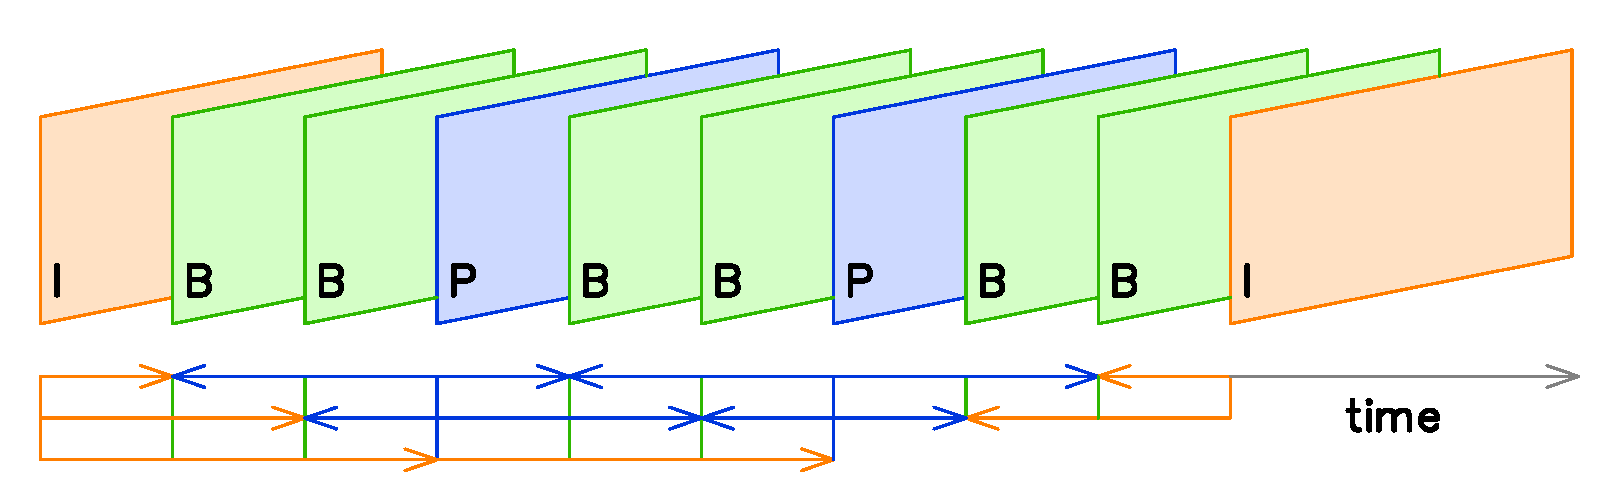
\includegraphics[width=0.95\textwidth]{figures-appconv2dash/gop-ipb.png}
  \caption{Example of a GOP structure (\href{http://en.wikipedia.org/wiki/Inter_frame}{Wikipedia}).}\label{fig:gopipb}
\end{figure}

\section{参考}

\subsection{split media files}
How to split a video using FFMPEG so that each chunk starts with a key frame?
\url{http://stackoverflow.com/questions/14005110/how-to-split-a-video-using-ffmpeg-so-that-each-chunk-starts-with-a-key-frame}



1. Jan 30 at 6:25
The latest builds of FFMPEG include a new option "segment" which does exactly what I think you need.
\begin{lstlisting}[language=bash]
ffmpeg -i INPUT.mp4 -acodec copy -f segment -vcodec copy -reset_timestamps 1 -map 0 OUTPUT%d.mp4
\end{lstlisting}
This produces a series of numbered output files which are split into segments based on Key Frames. In my own testing, it's worked well, although I haven't used it on anything longer than a few minutes and only in MP4 format.



2. Jul 16 '13 at 22:58
Using a newer build of ffmpeg, can achieve this by using ffprobe and the ffmpeg segment muxer.

1.Use ffprobe and awk to identify the keyframes as close as possible to your desired chunk length.
\begin{lstlisting}[language=bash]
ffprobe -show_frames -select_streams v:0 -print_format csv **[SOURCE_VIDEO]** 2>&1 | grep -n frame,video,1 | awk 'BEGIN { FS="," } { print $1 " " $5 }' | sed 's/:frame//g' | awk 'BEGIN { previous=0; frameIdx=0; size=0; } { split($2,time,"."); current=time[1]; if (current-previous >= **[DURATION_IN_SECONDS]**){ a[frameIdx]=$1; frameIdx++; size++; previous=current;} } END { str=a[0]; for(i=1;i<size;i++) { str = str "," a[i]; } print str;}'
\end{lstlisting}
Where
\begin{lstlisting}[language=bash]
    [SOURCE_VIDEO] = path to video you want to segment
    [DURATION_IN_SECONDS] = desired segment length in seconds
\end{lstlisting}
The output is comma-delimited string of keyframes.

2.Use the keyframes output above as input to ffmpeg.
\begin{lstlisting}[language=bash]
ffmpeg -i [SOURCE_VIDEO] -codec copy -map 0 -f segment -segment_frames [OUTPUT_OF_STEP_1] [SEGMENT_PREFIX] _%03d.[SOURCE_VIDEO_EXTENSION]
\end{lstlisting}
Where
\begin{lstlisting}[language=bash]
    [SOURCE_VIDEO] = path to video you want to segment
    [OUTPUT_OF_STEP_1] = comma-delimited string of keyframes
    [SEGMENT_PREFIX] = name of segment output
    [SOURCE_VIDEO_EXTENSION] = extension of source video (e.g., mp4, mkv)
\end{lstlisting}



3. Dec 23 '12 at 18:17
Here is the solution that I could get to work:

As suggested by av501 and d33pika, I used ffprobe to find where the key frames are. Because ffprobe is very verbose and can take several seconds or even minutes to output all key frames and there is no way to scope the range of frames we want from a lengthy video, I proceed into 5 steps:

    Export a video chunk from the original file, around the double of the desired chunk size.
\begin{lstlisting}[language=bash]
ffmpeg -i source.wmv -ss 00:00:00 -t 00:00:06 -acodec copy -vcodec copy -async 1 -y  0001.wmv
\end{lstlisting}
    Use ffprobe to find where the keyframes are. Choose closest keyframe after desired chunk size.
\begin{lstlisting}[language=bash]
ffprobe -show_frames -select_streams v -print_format json=c=1 0001.wmv
\end{lstlisting}
    From the output of ffprobe get the \texttt{pkt\_dts\_time} of the frame just before that key frame.

    ffmpeg on the exported chunk of step 1, specifying the same input and output file, and specifying -ss 00:00:00 and -t [value found in step 3].
\begin{lstlisting}[language=bash]
ffmpeg -i 0001.wmv -ss 00:00:00 -t 00:00:03.1350000 -acodec copy -vcodec copy -async 1 -y 0001.wmv
\end{lstlisting}
    Restart at step 1, using -ss [cumulated sum of values found in step 3 over iterations].

Proceeding this way, I was able to have an efficient and robust way to split the video at key frames.



4. Dec 23 '12 at 14:11
Use ffprobe -show\_frames -pretty <stream> to identify the key frames.


5. Dec 23 '12 at 3:36
If you are willing to do some scripting and want I frames at a particular interval the one way to do it is

Run ffprobe and collect the locations of the I frames from the output
\begin{lstlisting}[language=bash]
ffprobe -show_streams
\end{lstlisting}
Run a series of -ss -t commands using the same script to get the chunks you desire.

You can then have your script decide minimum number of frames [say there are two I pictures within 10 frames of each other, you really don't want to be chunking it there].

\chapter{References}

Google MapReduce for C: Run Native Code in Hadoop
\url{http://google-opensource.blogspot.com/2015/02/mapreduce-for-c-run-native-code-in.html}



Cloud MapReduce -- A MapReduce implementation on Amazon Cloud OS
\url{https://code.google.com/p/cloudmapreduce/}


Apache Storm is a free and open source distributed realtime computation system.
\url{http://storm.apache.org/}

Apache Spark is a fast and general engine for large-scale data processing.
\url{http://spark.apache.org/}


\section{C/C++}


\href{http://hypertable.com/}{Hypertable} is a high performance, open source, massively scalable database modeled after Bigtable, Google's proprietary, massively scalable database.

\section{python}


\href{https://github.com/mfisk/filemap.git}{FileMap} is a file-based map-reduce system for data-parallel computation. (python)

\href{https://code.google.com/p/octopy/}{octopy} Easy MapReduce for Python

\href{https://github.com/michaelfairley/mincemeatpy.git}{mincemeatpy} Lightweight MapReduce in python (2013)

\href{http://heynemann.github.io/r3/}{r³} is a map reduce engine written in python using a redis backend. It's purpose is to be simple.


\href{http://discoproject.org/}{Disco} is a lightweight, open-source framework for distributed computing based on the MapReduce paradigm.



\url{https://wiki.python.org/moin/ParallelProcessing}
python Parallel Processing

\href{http://ipython.org/}{IPython} provides tools for interactive and parallel computing that are widely used in scientific computing, but can benefit any Python developer.

\section{Bash}

bashreduce (origin) \url{https://github.com/erikfrey/bashreduce.git}

improved bashreduce \url{https://github.com/dakusui/bredxbred.git},
or \url{https://github.com/rcrowley/bashreduce.git}. others, \href{https://github.com/jweslley/bashreduce.git}{jweslley}.



others:
\href{https://github.com/jasonMatney/BashMapReduce.git}{BashMapReduce},
\href{https://github.com/sorhus/bash-reduce.git}{bash-reduce},
\href{https://github.com/colestanfield/map-reduce.git}{map-reduce},
\href{https://github.com/argent0/mr-tools.git}{mr-tools},


\section{others}



\url{http://quantcast.github.io/qfs/}
Quantcast File System (QFS) is a high-performance, fault-tolerant, distributed file system developed to support MapReduce processing, or other applications reading and writing large files sequentially.

\href{https://rubygems.org/gems/mapredus}{mapredus}, simple mapreduce framework using redis and resque

\href{http://projects.camlcity.org/projects/plasma.html}{Plasma}: Distributed filesystem, key/value db, and map/reduce system. 2011


\href{http://mapreduce.sandia.gov/}{MapReduce-MPI Library} includes C++ and C interfaces callable from most hi-level languages, and also a Python wrapper


\href{http://sector.sourceforge.net/}{Sector/Sphere} is a system for distributed data storage, distribution, and processing. The system works on clusters of commodity computers. Sector provides client tools to access data stored in the system and API for the development of distributed data processing applications.

\href{http://skynet.rubyforge.org/}{Skynet} is an open source Ruby implementation of Google’s MapReduce framework


\href{https://code.google.com/p/httpmr/}{httpmr} A scalable data processing framework for people with web clusters


\href{https://code.google.com/p/qizmt/}{qizmt} is a mapreduce framework for executing and developing distributed computation applications on large clusters of Windows servers.




\href{https://code.google.com/p/cloudmapreduce/}{Cloud MapReduce} -- A MapReduce implementation on Amazon Cloud OS

\url{https://github.com/googlecloudplatform/appengine-mapreduce}
A library for running MapReduce jobs on App Engine




\url{https://github.com/documentcloud/cloud-crowd}
Write your scripts in Ruby, Works with Amazon EC2 and S3



\url{http://www.cse.ust.hk/gpuqp/Mars.html}
A MapReduce Framework on Graphics Processors


\url{https://github.com/ryanmcgrath/maprejuice}
javascript, node.js

\chapter{Source Code}

\begin{lstlisting}[language=bash]
ffprobe -show_streams
\end{lstlisting}


\end{document}



